%% 美赛模板:正文部分

\documentclass[12pt]{article}  % 官方要求字号不小于 12 号,此处选择 12 号字体
% 本模板不需要填写年份,以当前电脑时间自动生成
% 请在以下的方括号中填写队伍控制号
\usepackage[2321846]{easymcm}  % 载入 EasyMCM 模板文件
\problem{C}  % 请在此处填写题号
 \usepackage{mathptmx}  % 这是 Times 字体,中规中矩 
%\usepackage{mathpazo}  % 这是 COMAP 官方杂志采用的更好看的 Palatino 字体,可替代以上的 mathptmx 宏包
\title{\huge{\textbf{{\sc Our Title}}}\\ Our Title}  % 标题
\usepackage{enumerate}
\usepackage{lettrine}
\usepackage[ruled,linesnumbered]{algorithm2e}
\usepackage{lipsum}
\usepackage{hyperref}
\usepackage{adjustbox}
% 如需要修改题头(默认为 MCM/ICM),请使用以下命令(此处修改为 MCM)
%\renewcommand{\contest}{MCM}
\usepackage{bm}
\usepackage{cleveref}
\usepackage{ulem}
\usepackage{geometry}
\usepackage{framed} 
\usepackage{mathrsfs}
\usepackage{lettrine}
\usepackage{wasysym}
\usepackage[table,xcdraw]{xcolor}
% \usepackage{graphicx}%图片头文件
% \usepackage{float} %指定图片位置
% \usepackage{subfigure}
% 文档开始
\begin{document}

% 此处填写摘要内容
\begin{abstract}

    \vspace{5pt}
    \textbf{Keywords}:

\end{abstract}

\maketitle 
 % 生成 Summary Sheet
\tableofcontents
% 正文开始
\section{Introduction}
\subsection{Background}

\subsection{Restatement of the Problem}
\begin{enumerate}[\textbf{problem} 1 ]
\item text
\end{enumerate}
\subsection{Our Work}
{\LARGE\CheckedBox} 

 Here's our work:
\begin{figure}[htbp]
\centering
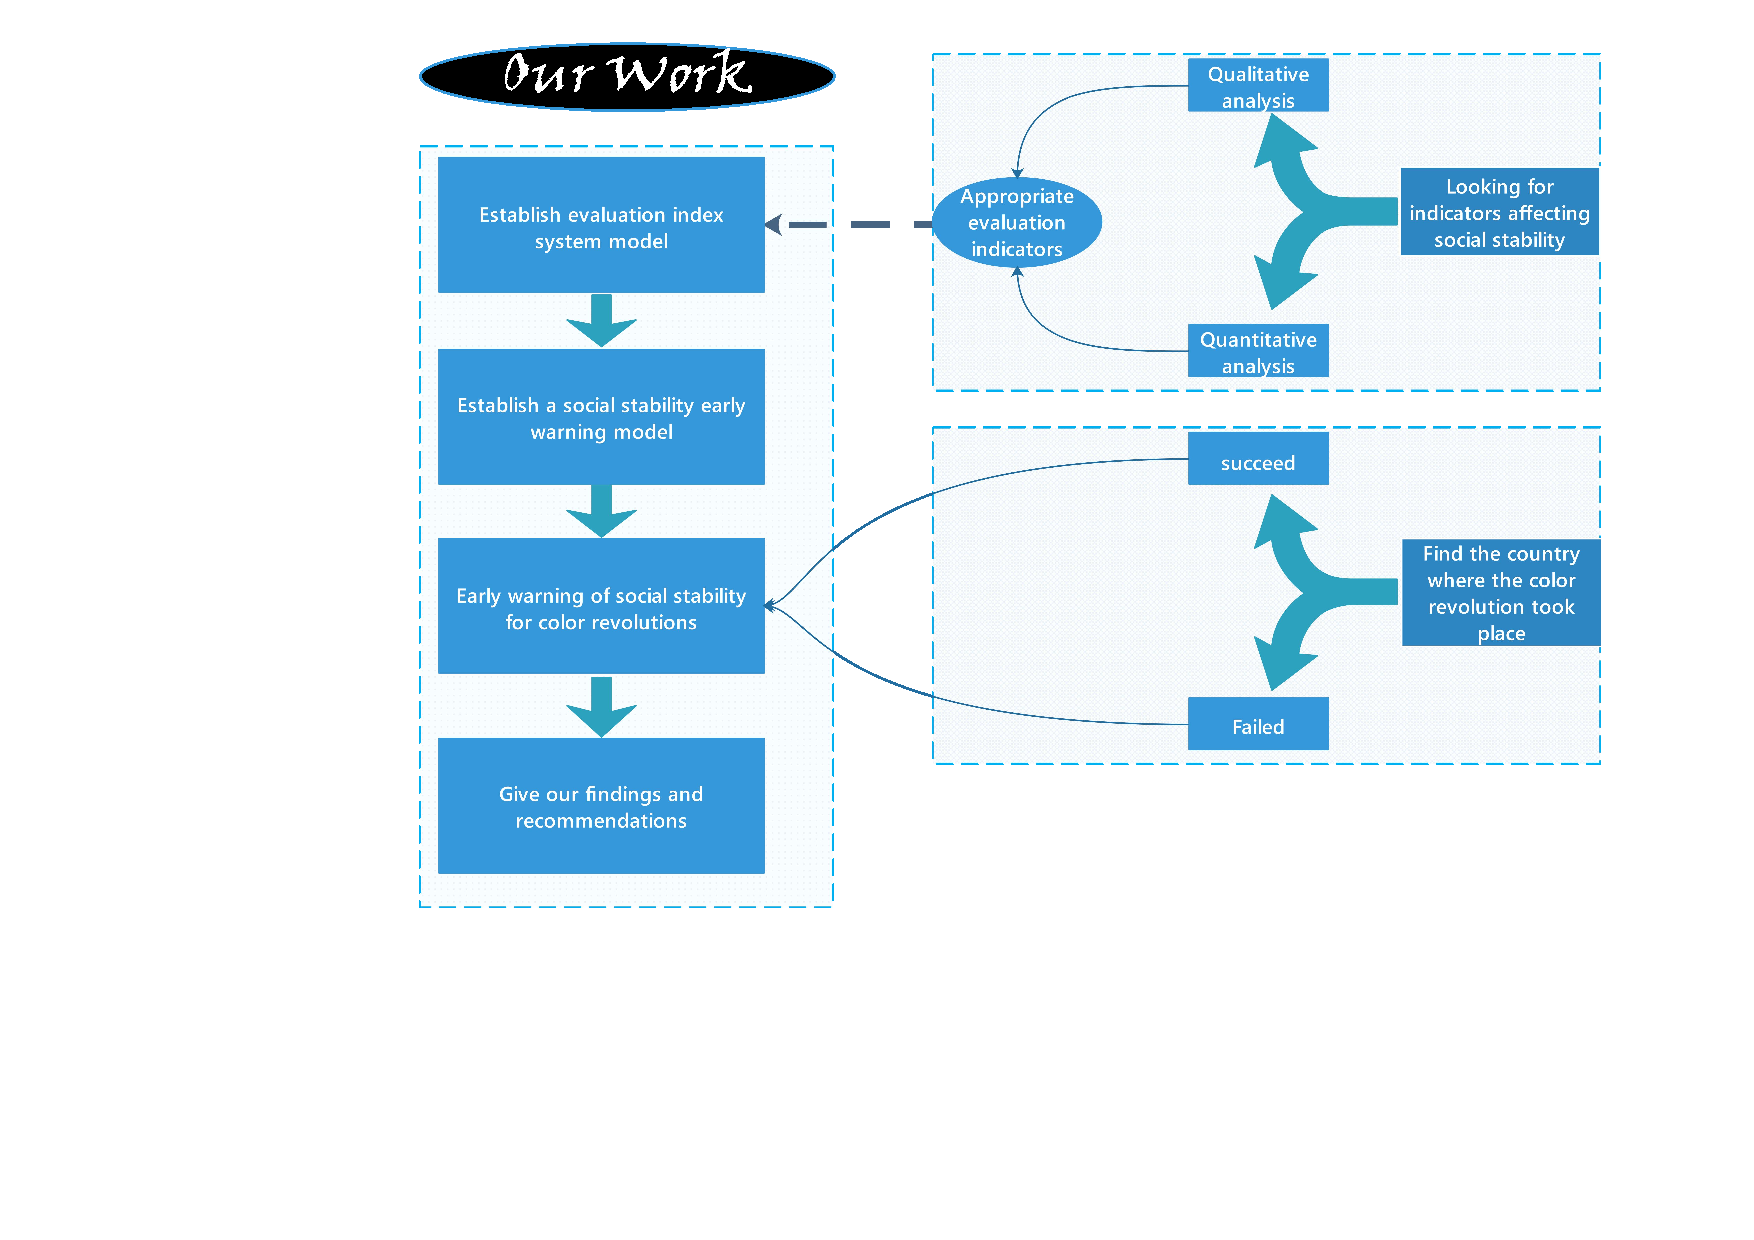
\includegraphics[width=.4\textwidth]{img/our work.pdf}
\caption{Our Work}
\end{figure}
\begin{figure}[htbp]
\centering
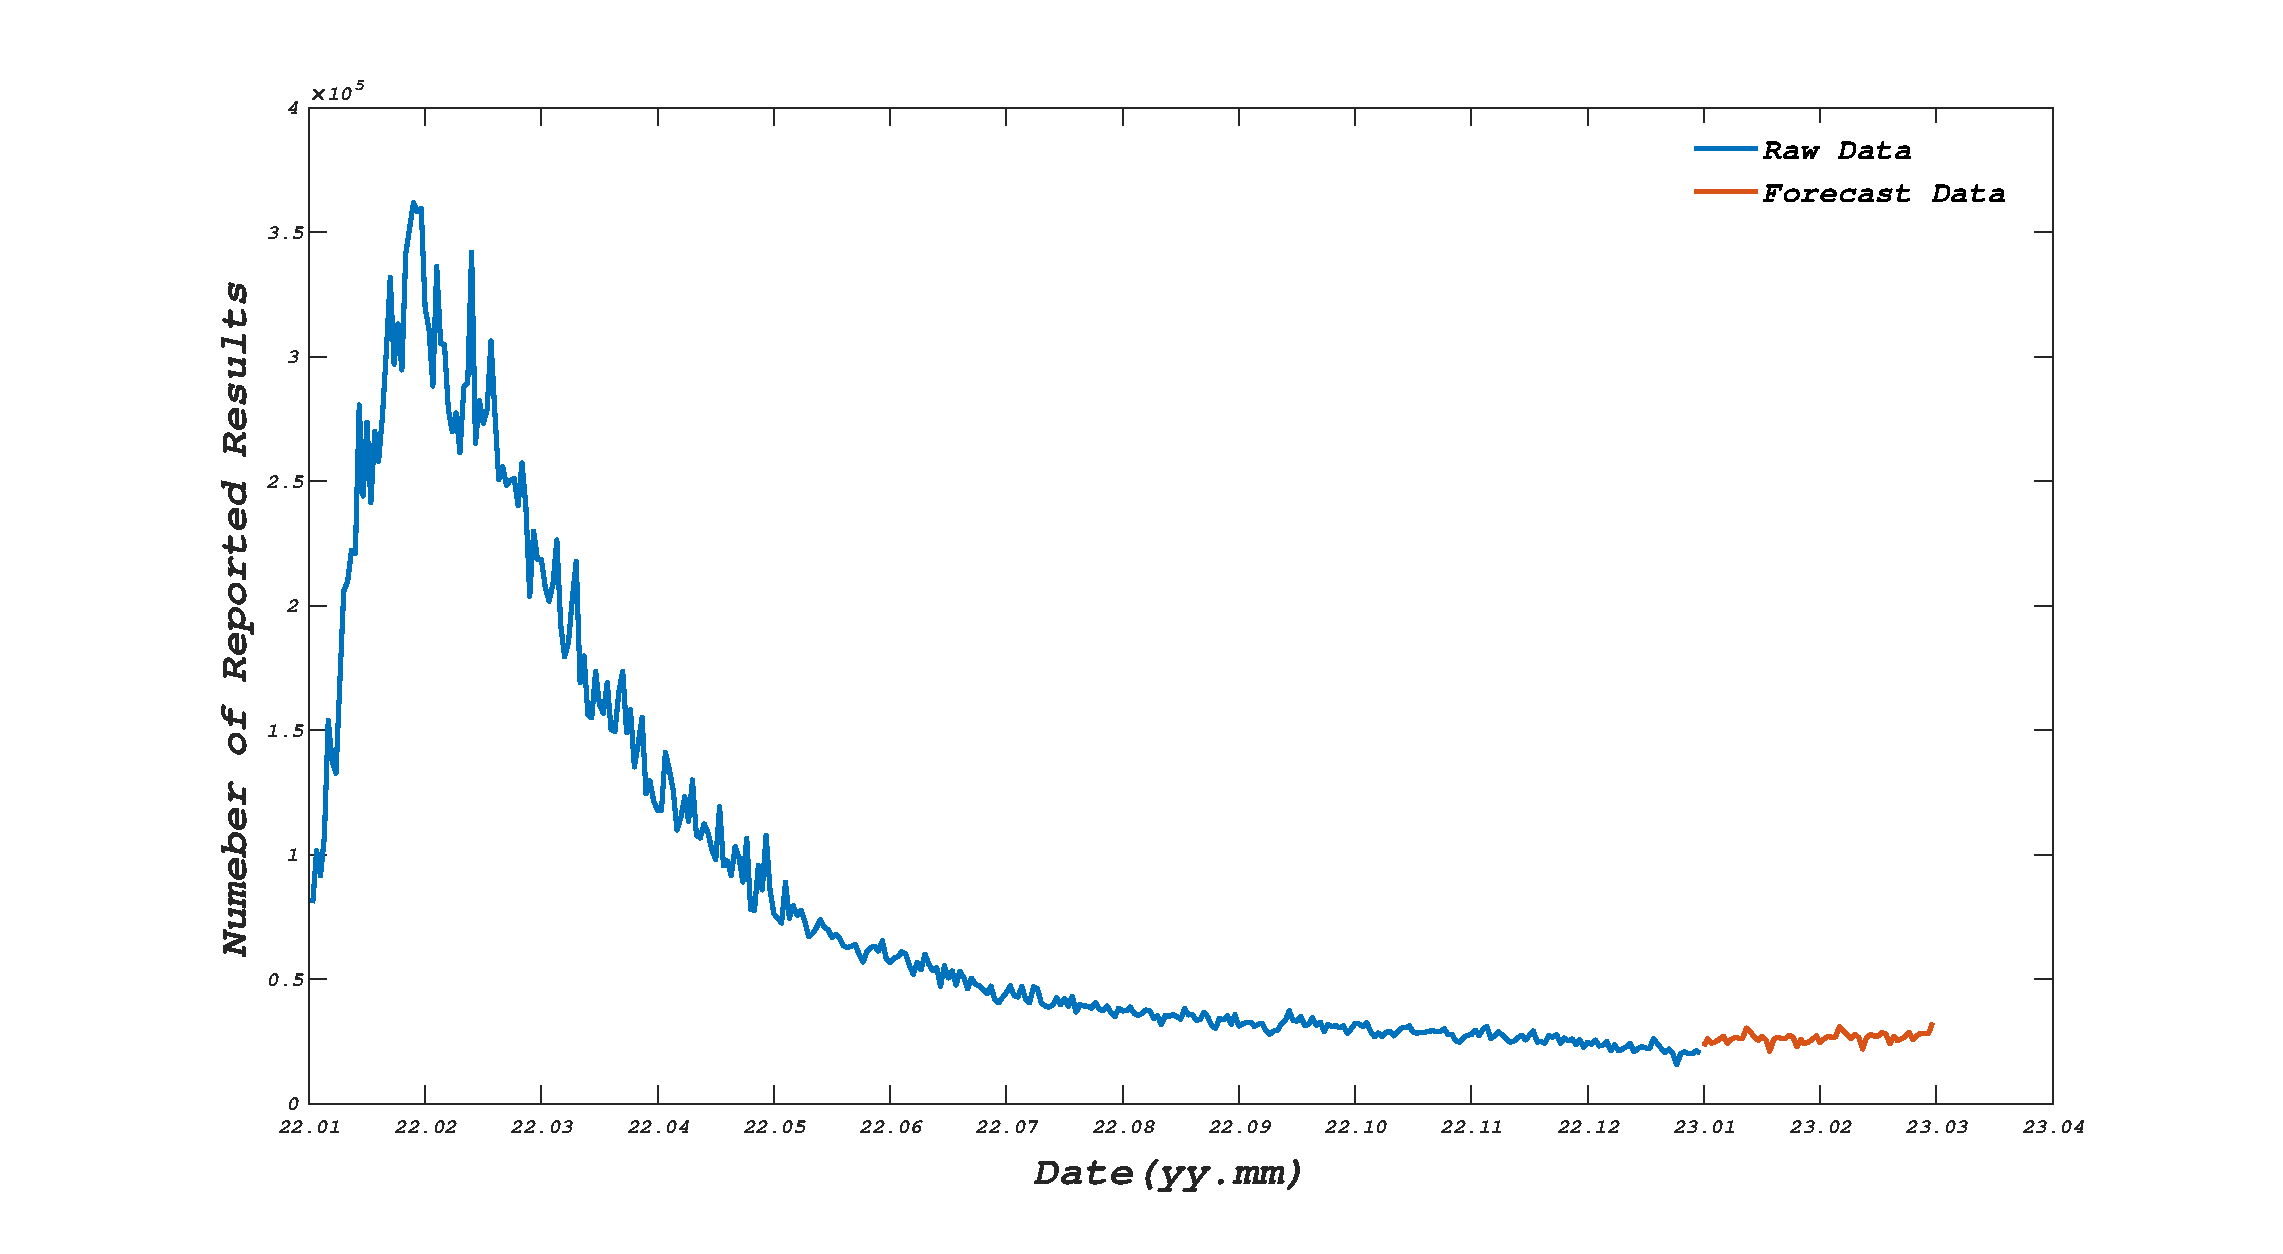
\includegraphics[width=\textwidth]{img/yuce.eps}
\caption{forecast}
\end{figure}
\begin{figure}[htbp]
\centering
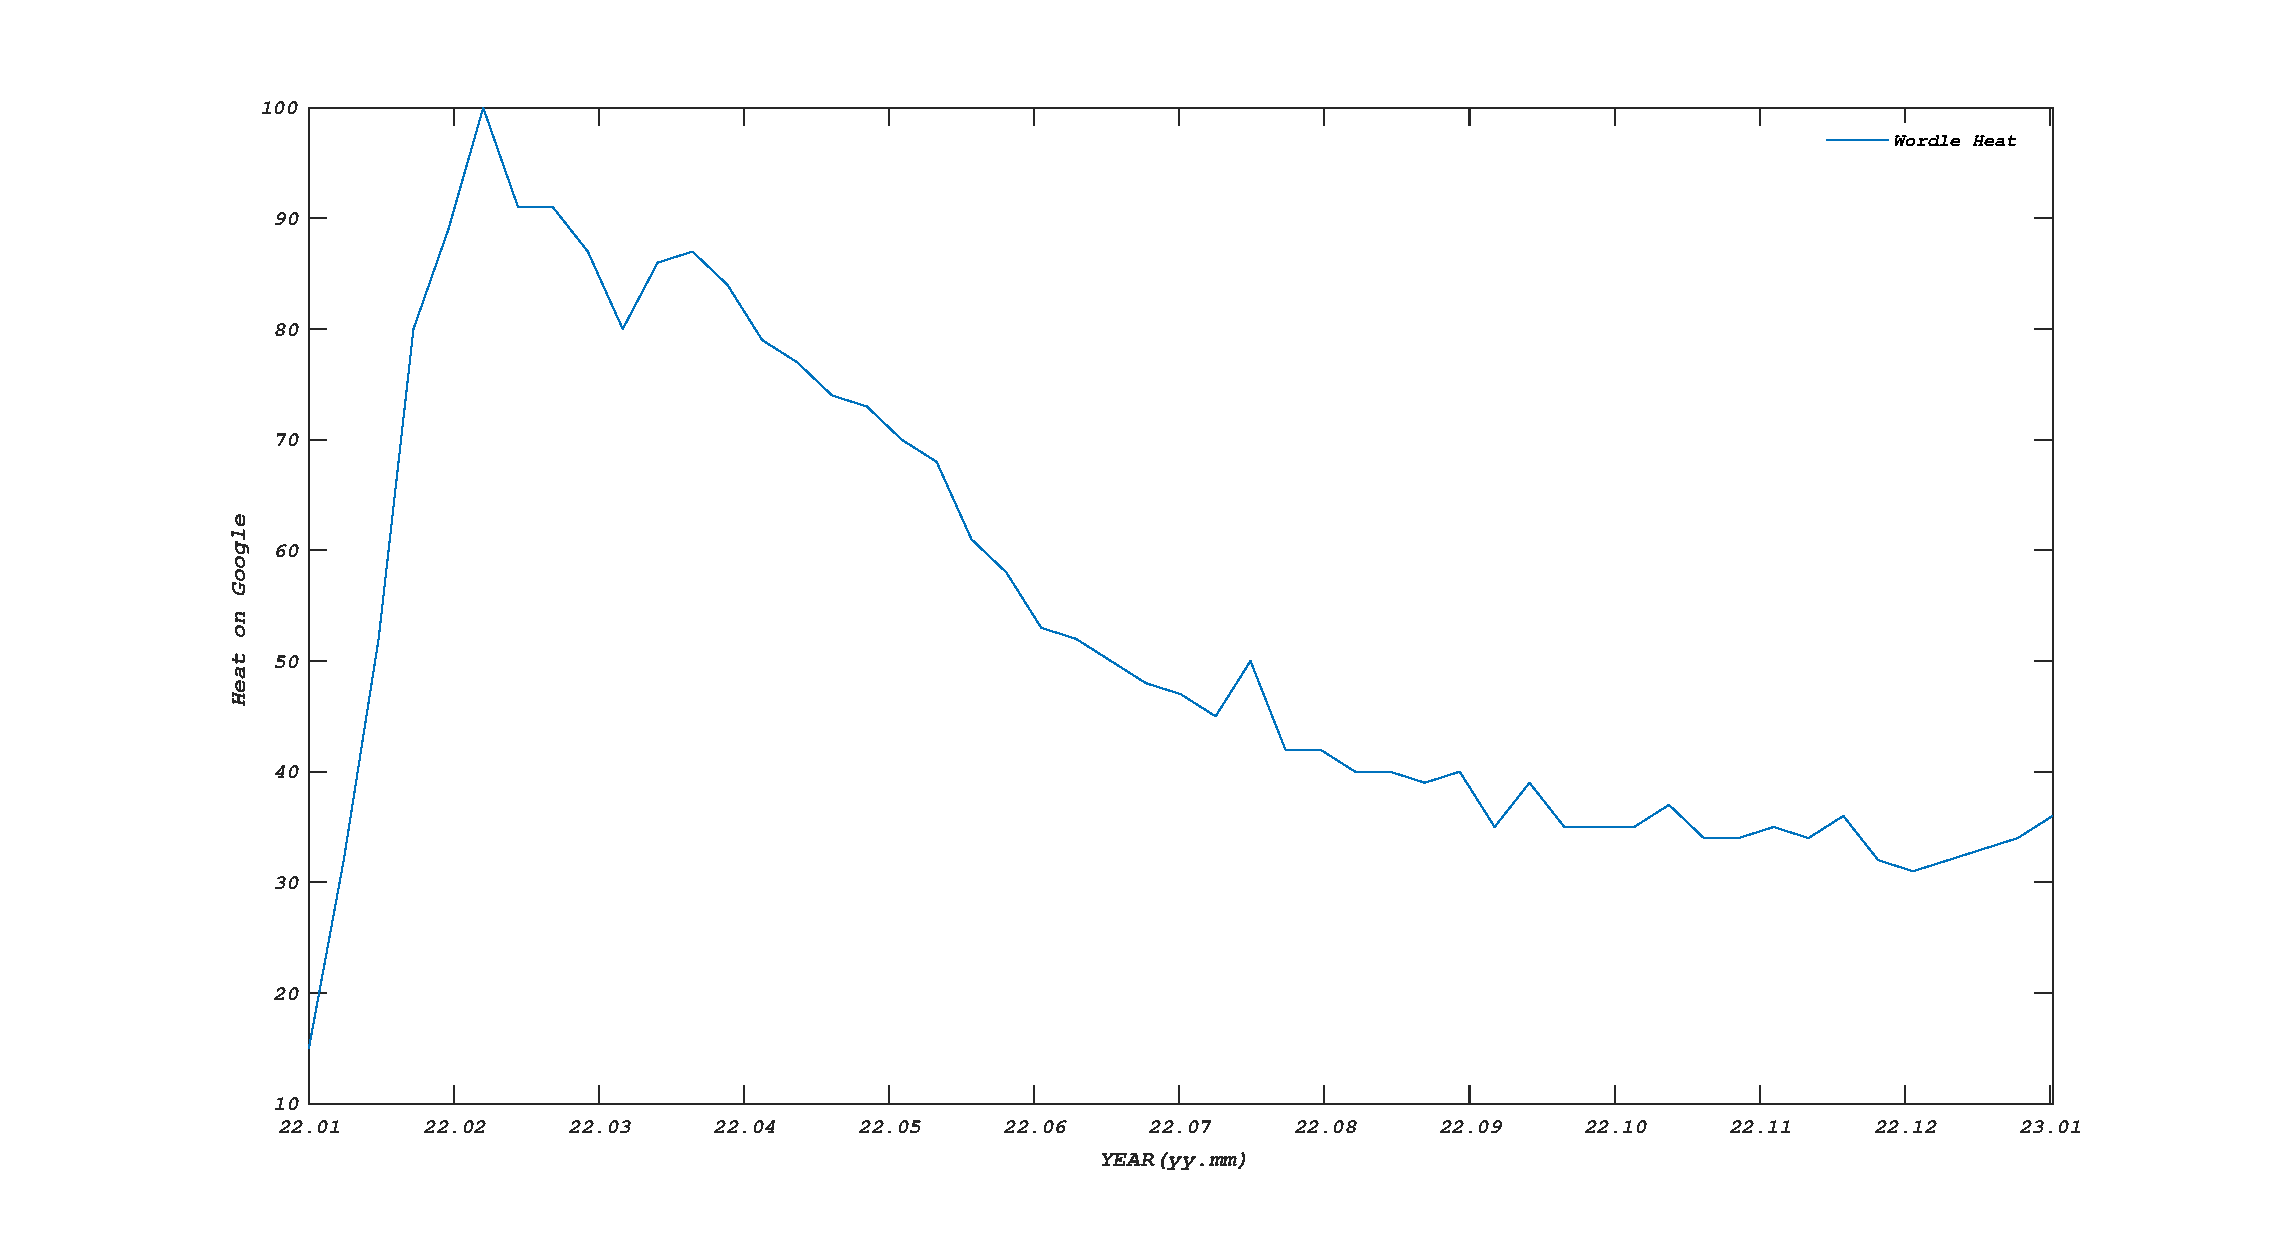
\includegraphics[width=\textwidth]{img/heat.eps}
\caption{heat}
\end{figure}
\begin{figure}[htbp]
\centering
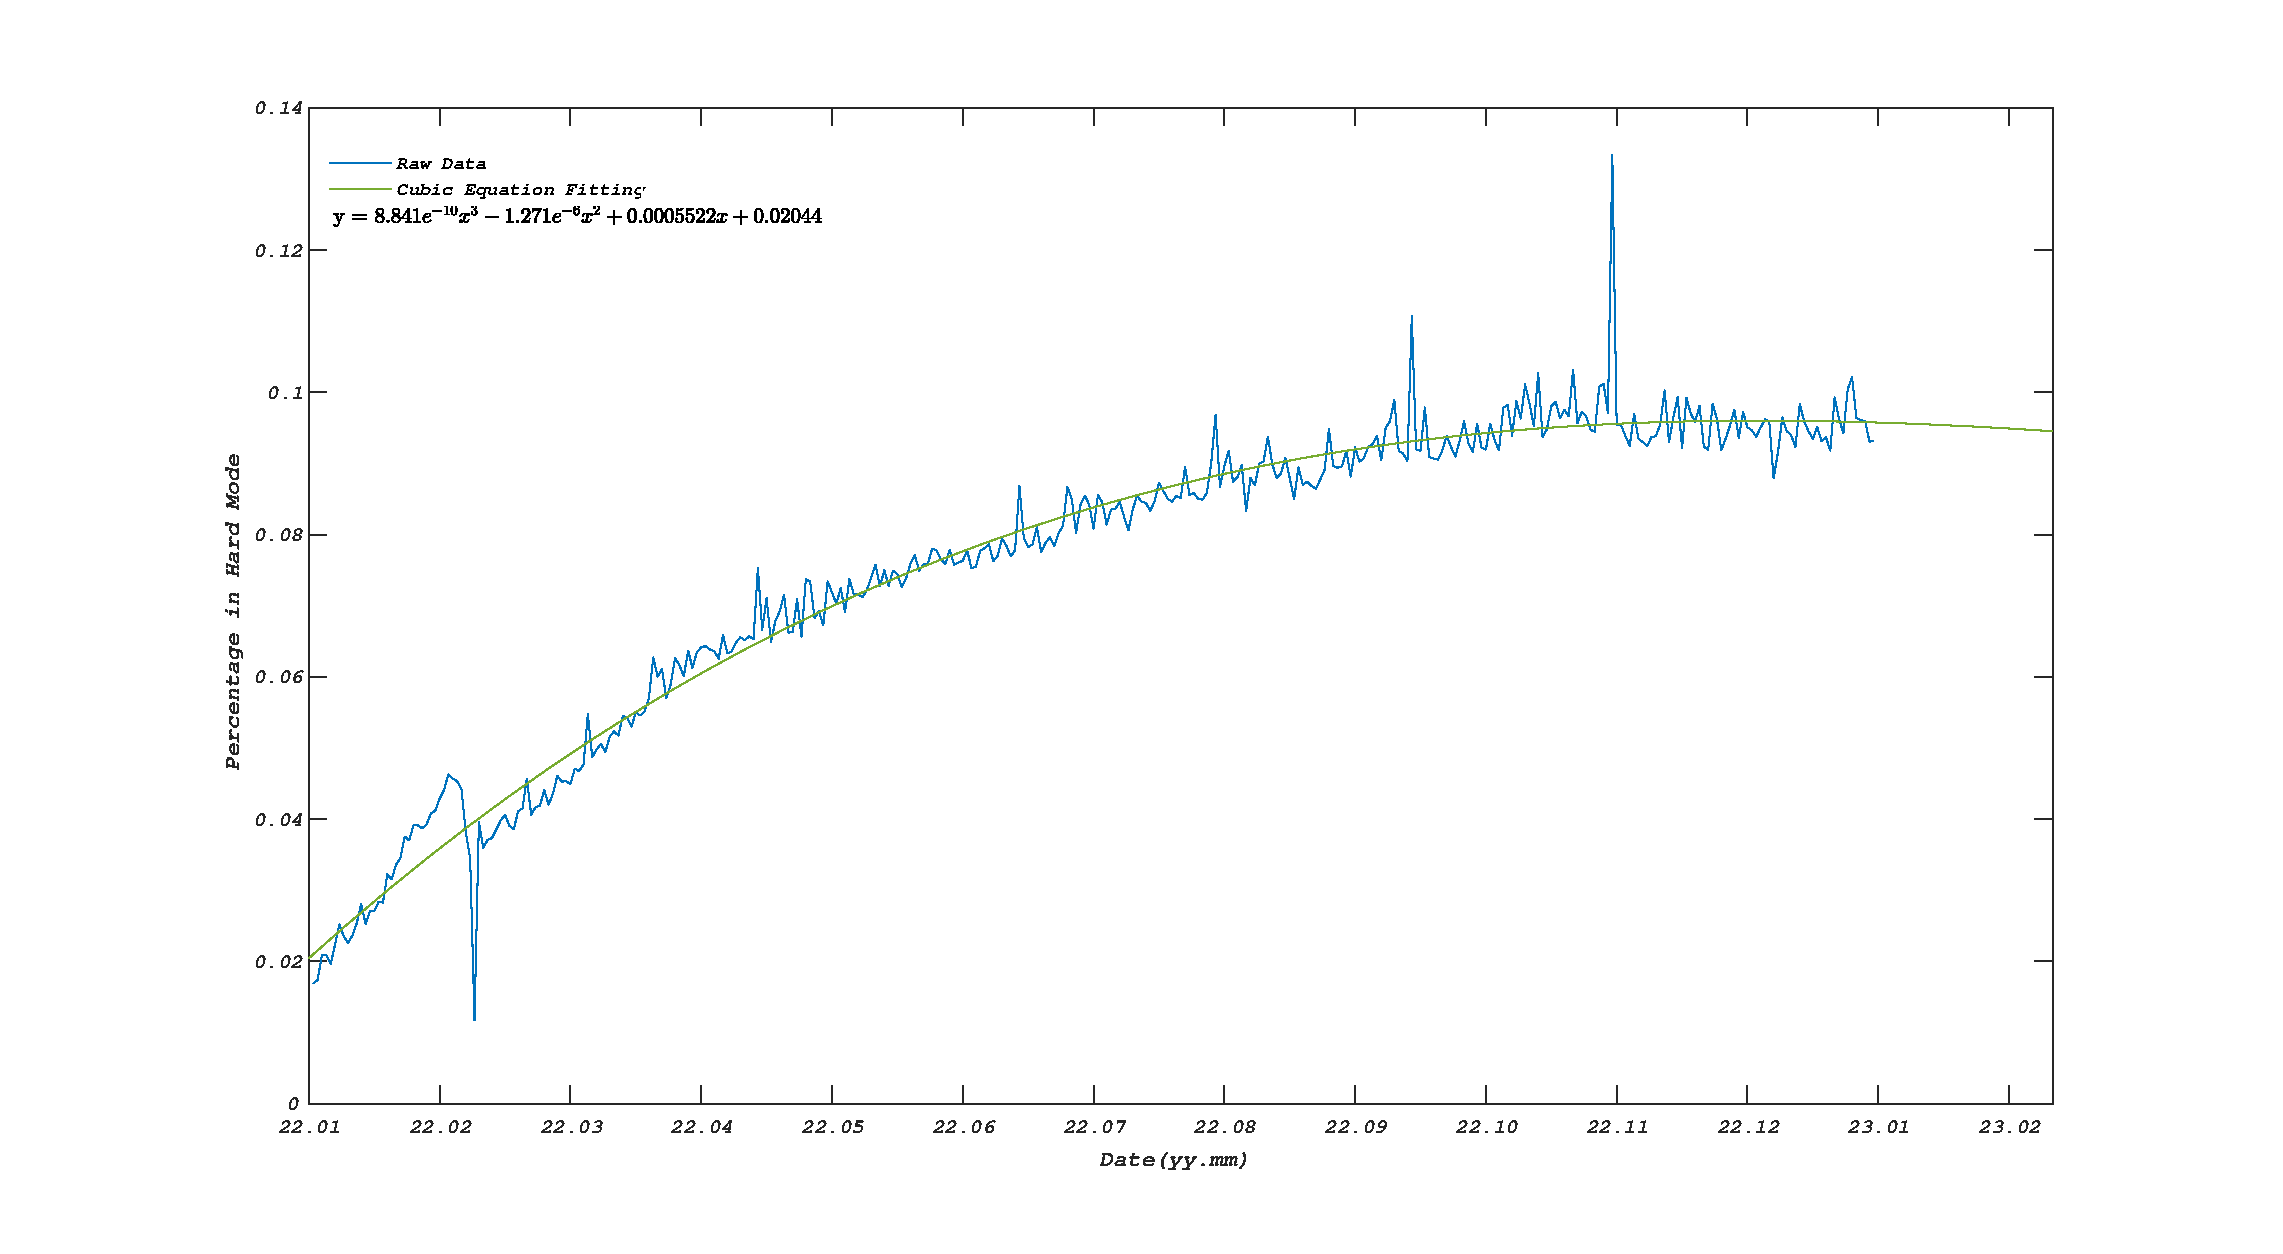
\includegraphics[width=\textwidth]{img/sanci.eps}
\caption{sanci}
\end{figure}
% \begin{figure}[htbp]
% \centering
% 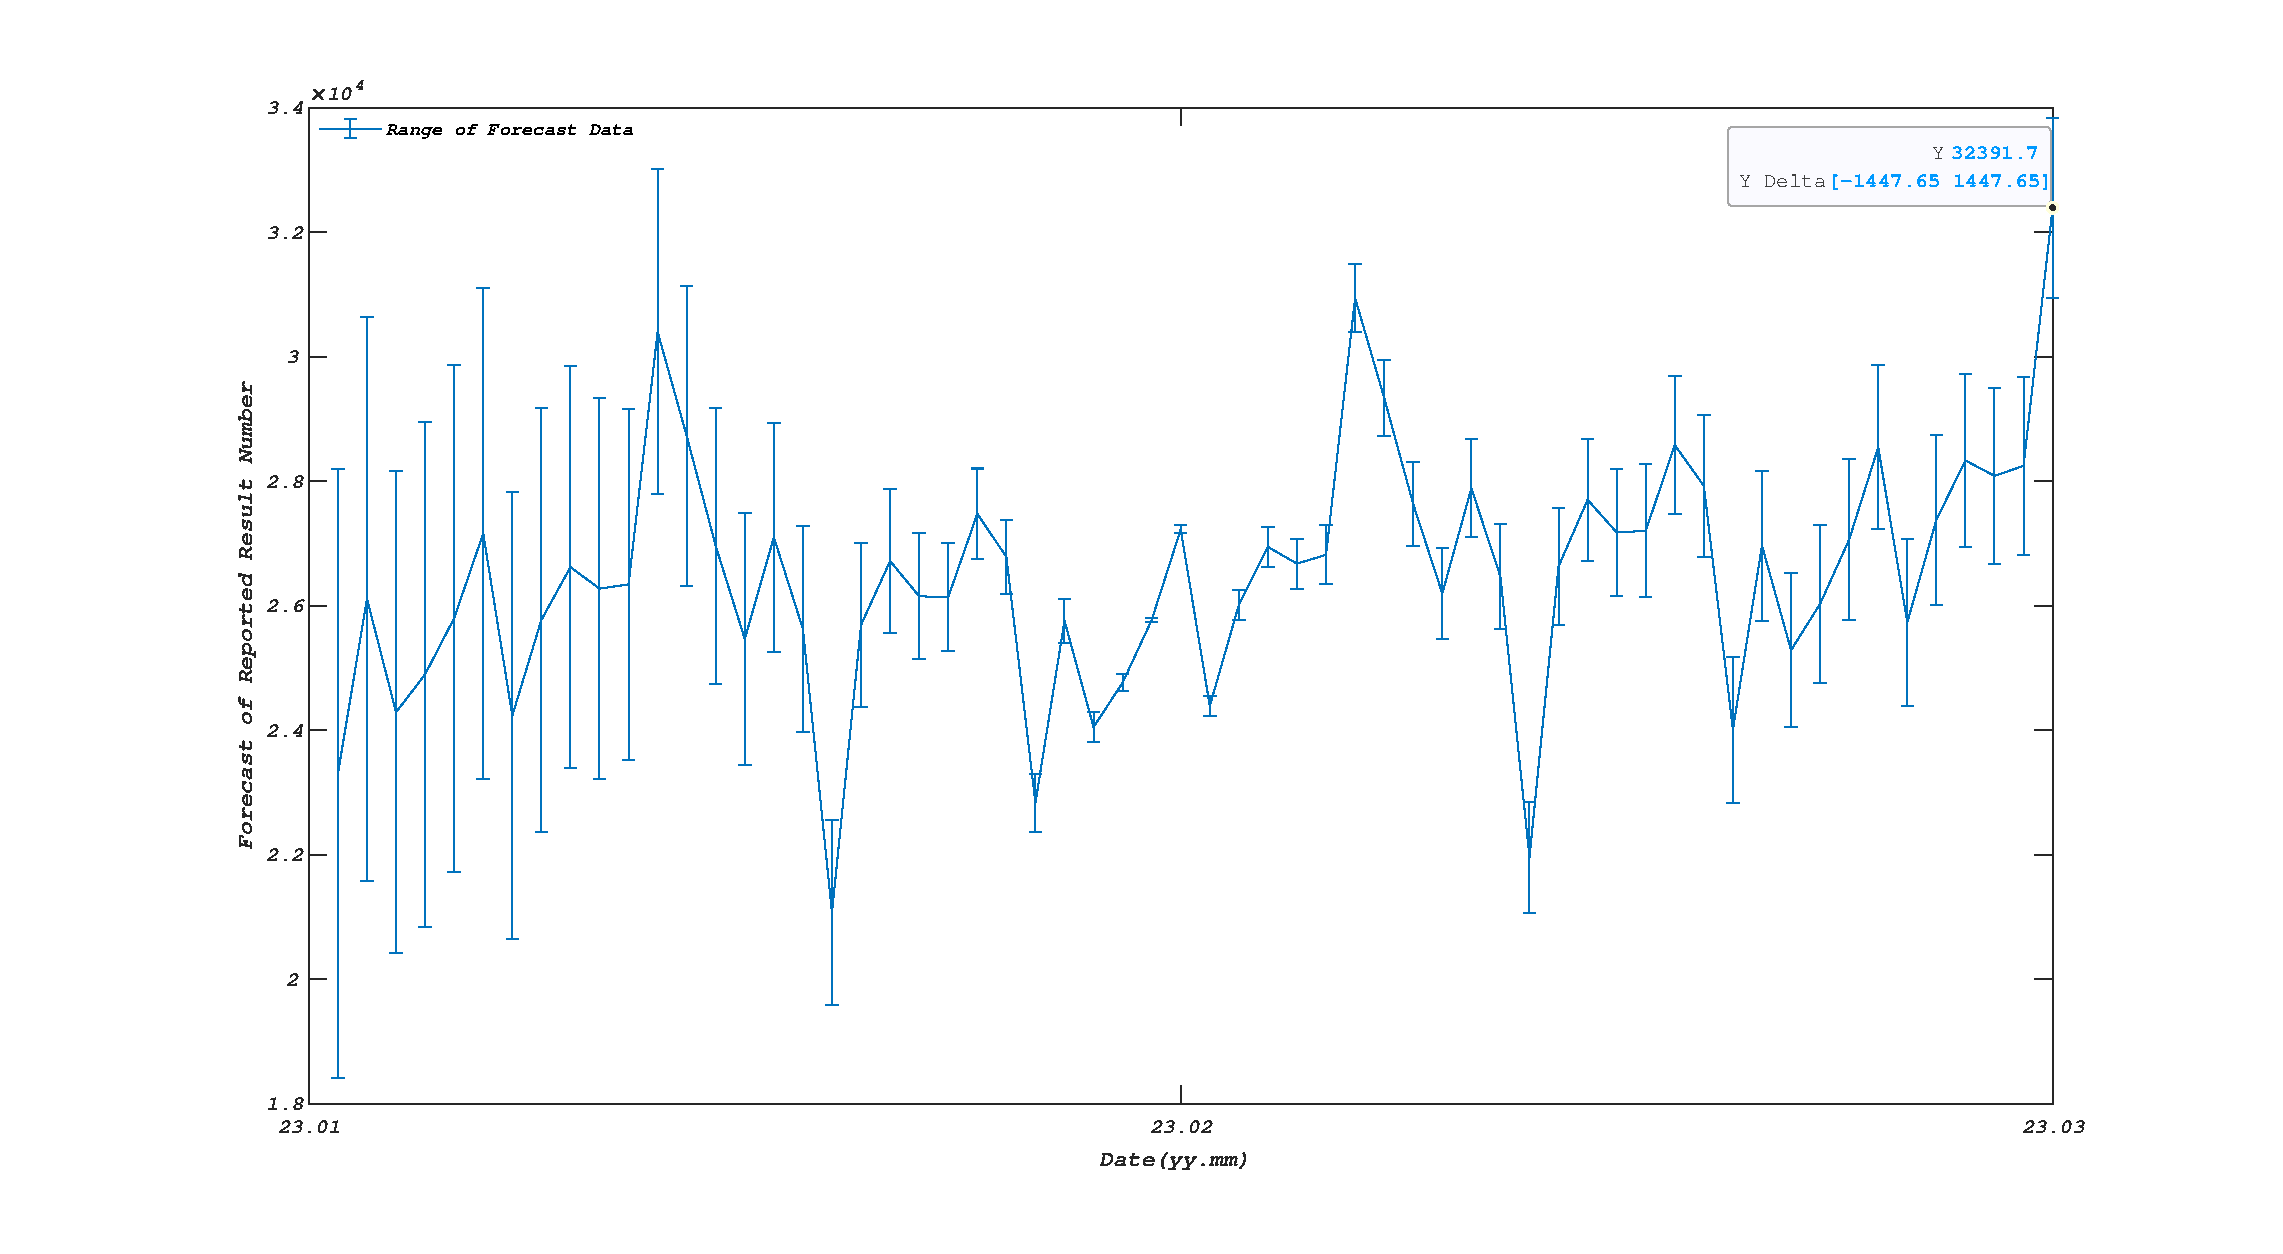
\includegraphics[width=\textwidth]{img/wucha.eps}
% \caption{wucha}
% \end{figure}
% \begin{figure}[htbp]
% \centering
% 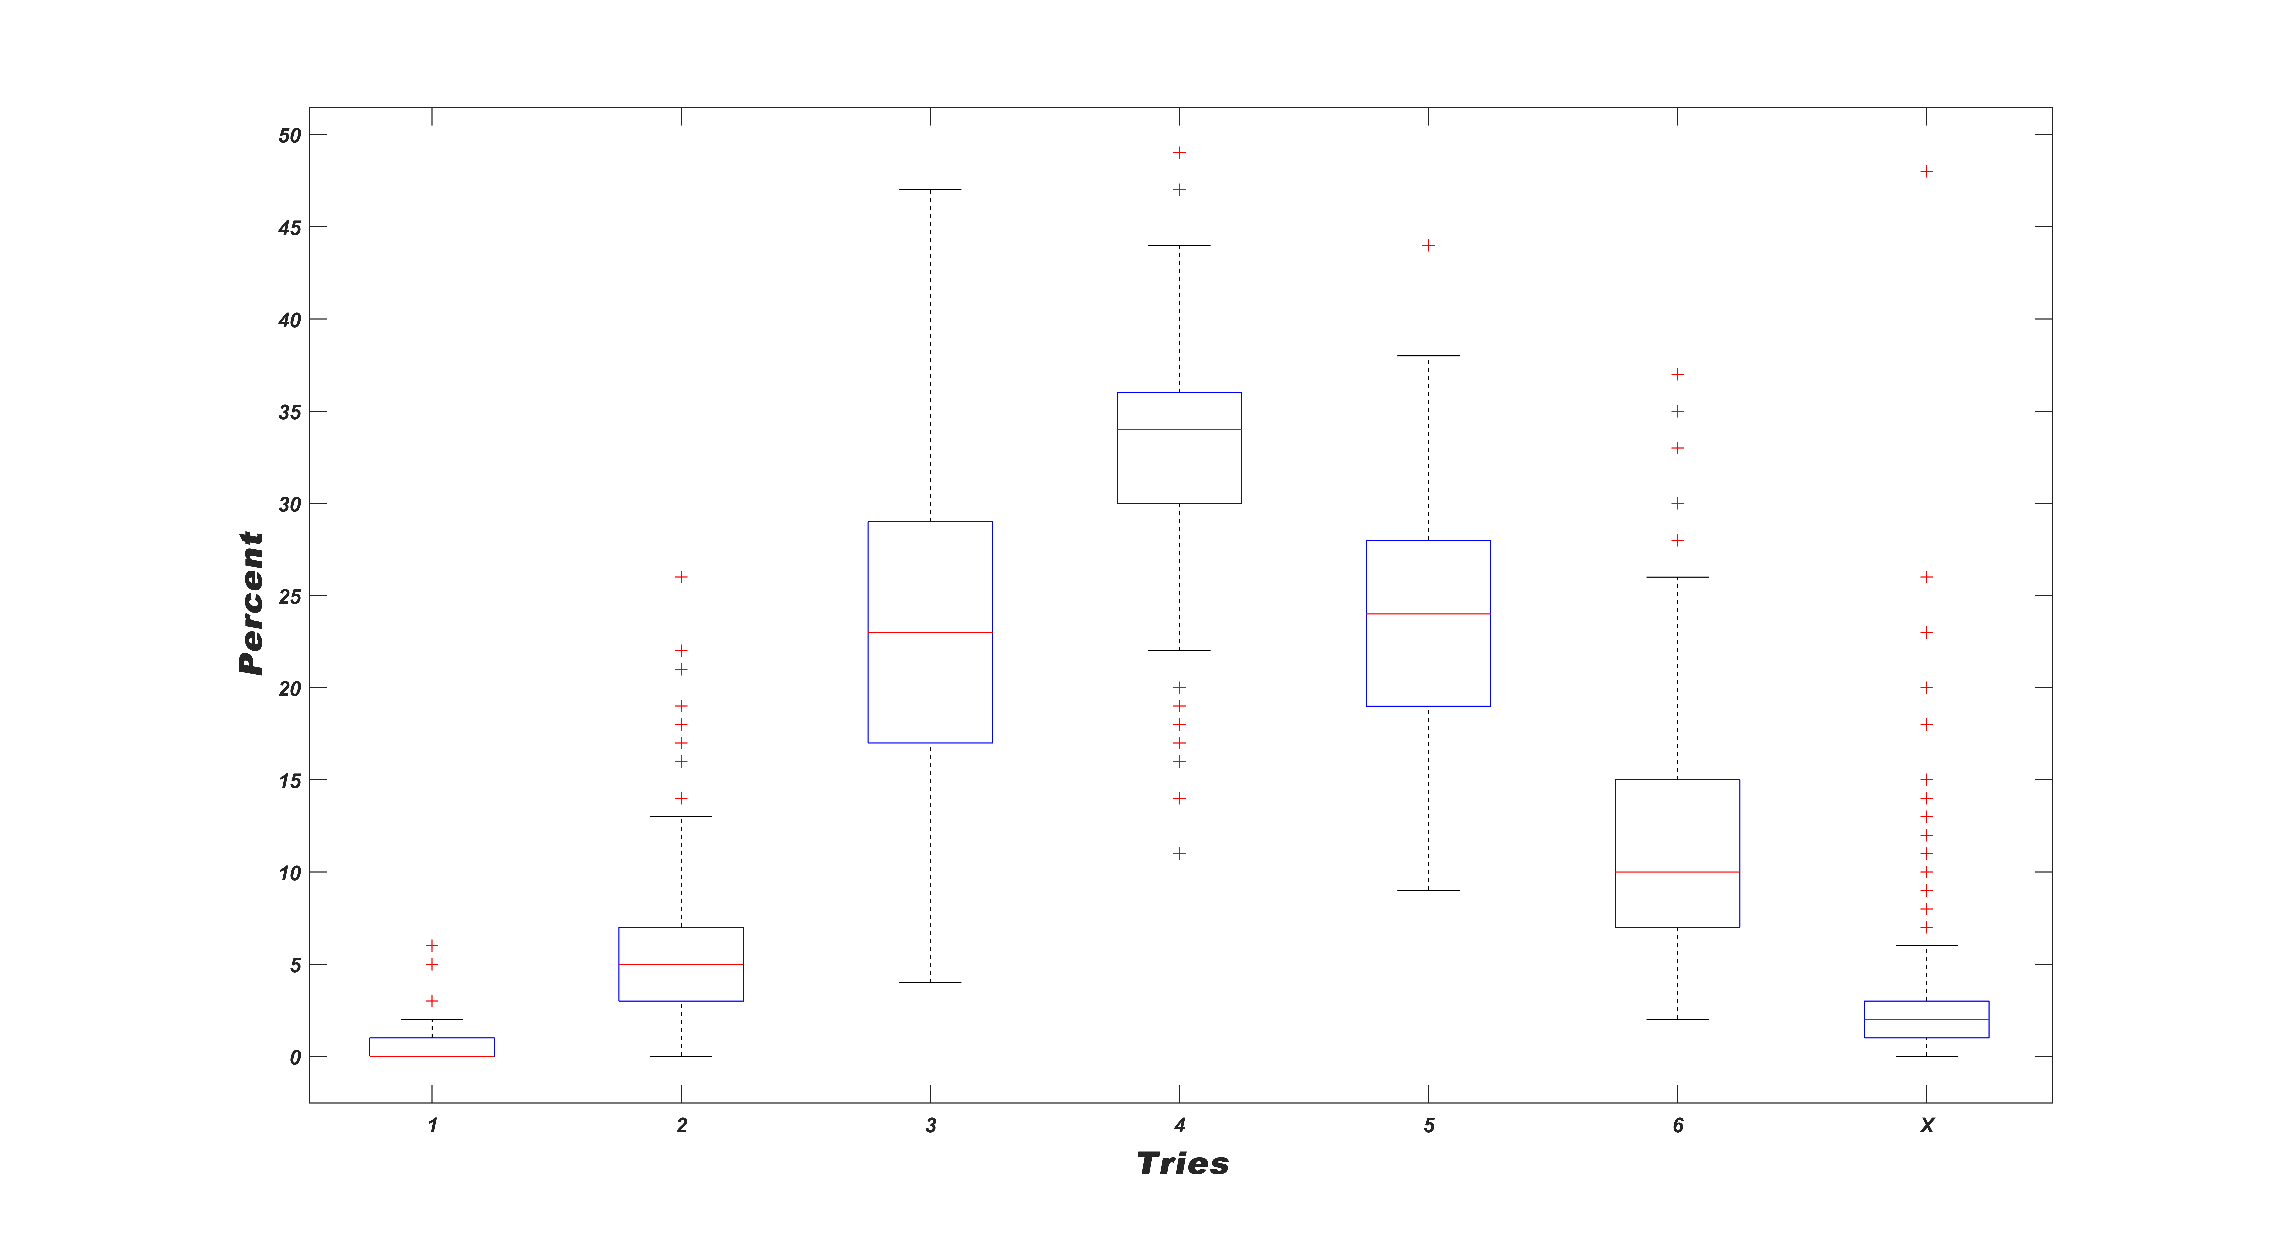
\includegraphics[width=\textwidth]{img/xxt.eps}
% \caption{xxt}
% \end{figure}
\begin{figure}[htbp]
\centering
\begin{subfigure}[b]{.49\textwidth}
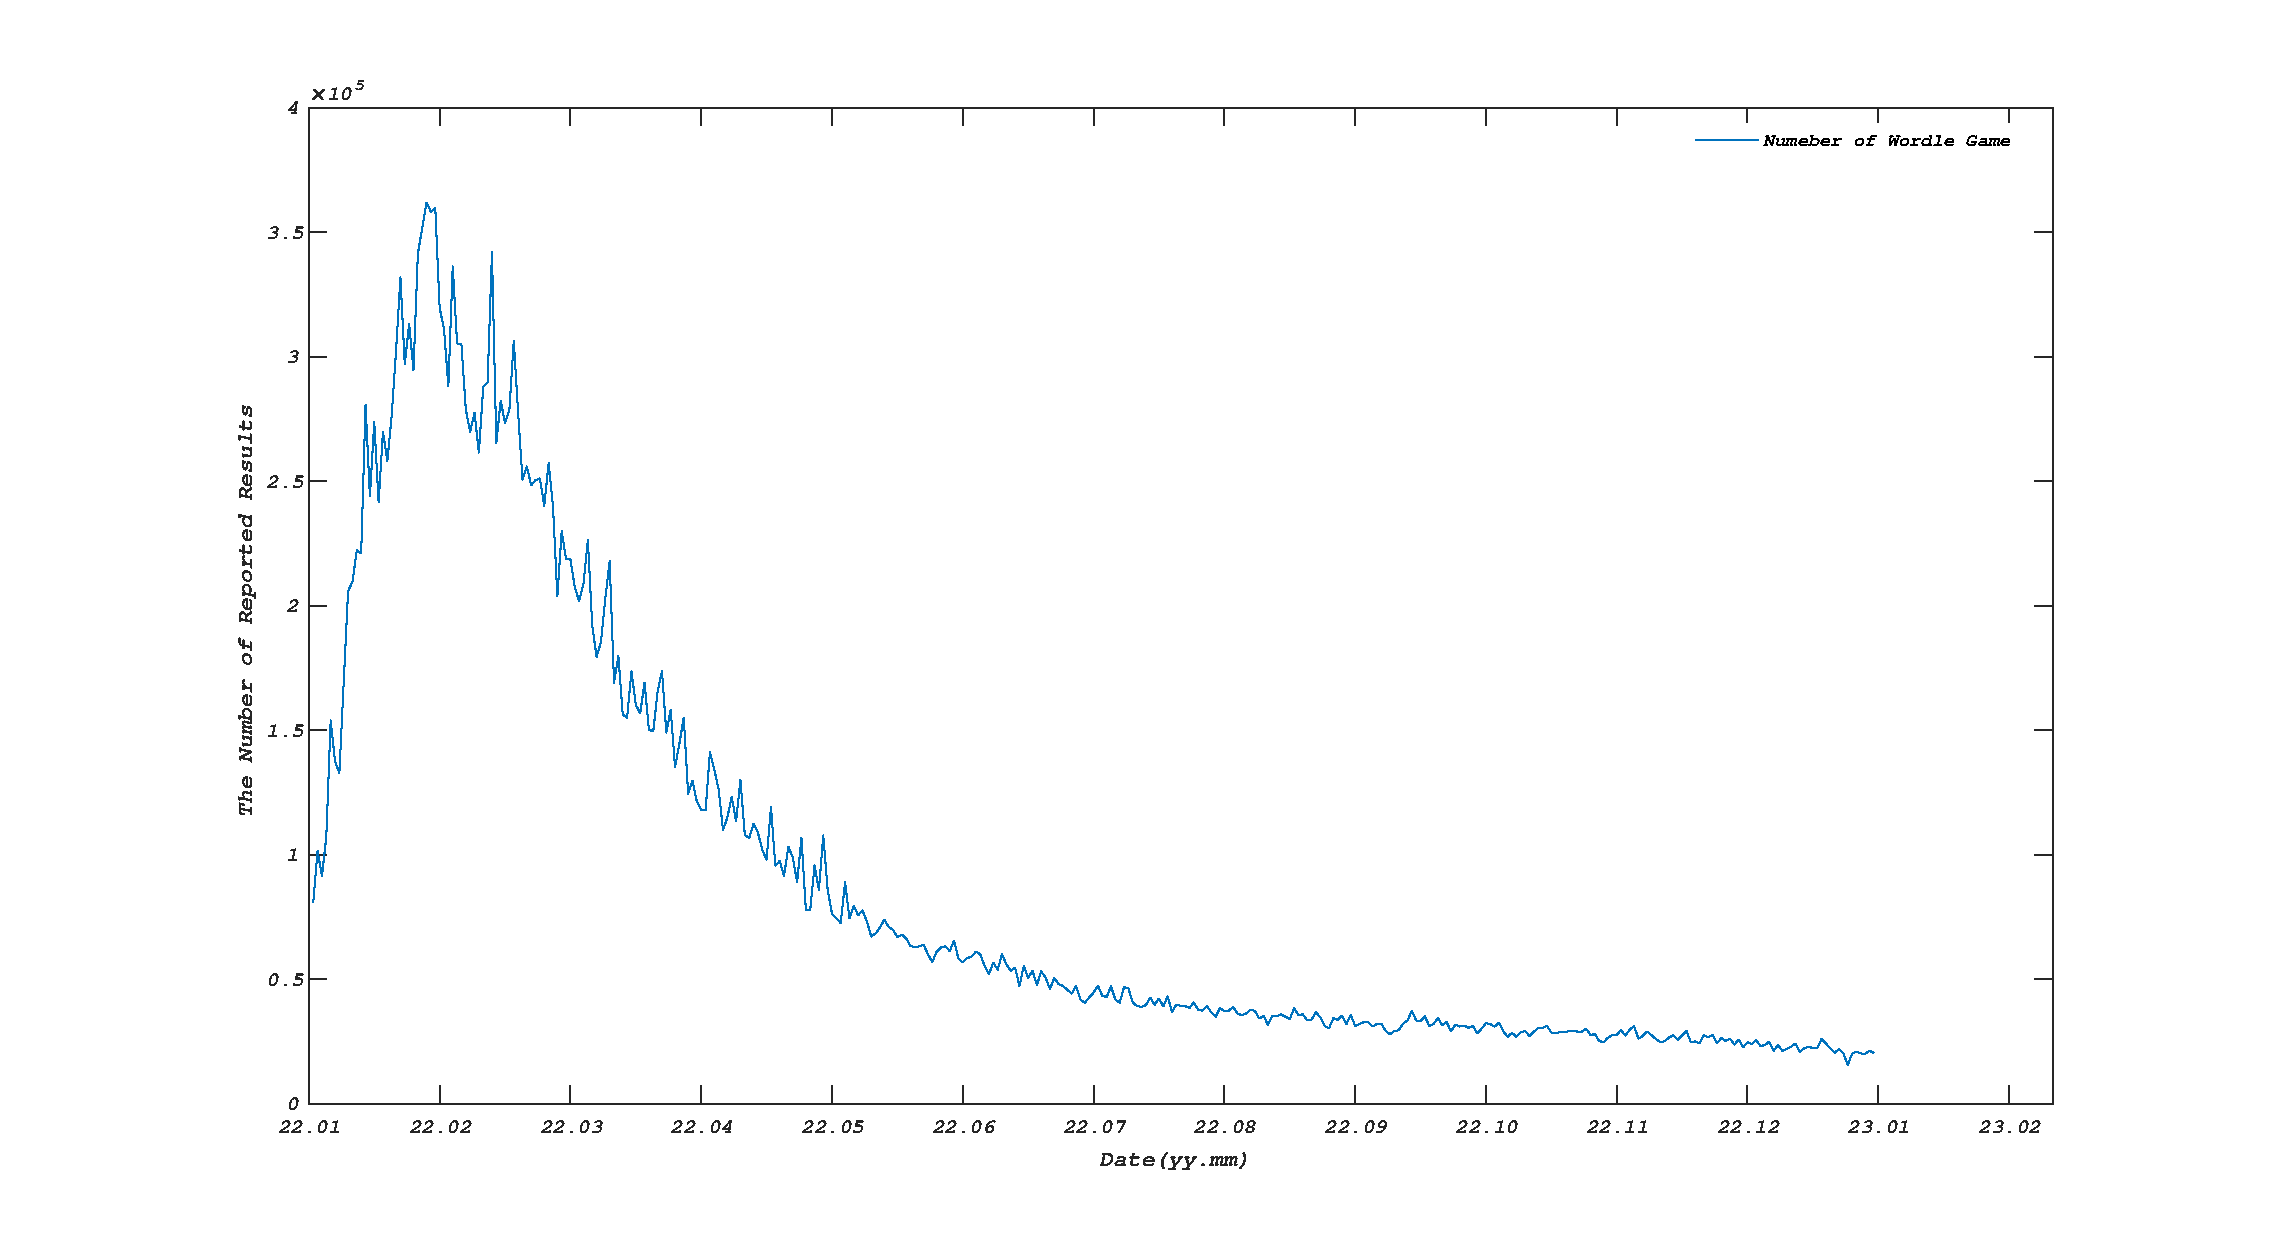
\includegraphics[width=\textwidth]{img/yuanshi.eps}\caption{The Number of Reported Results}
\end{subfigure}
\begin{subfigure}[b]{.49\textwidth}
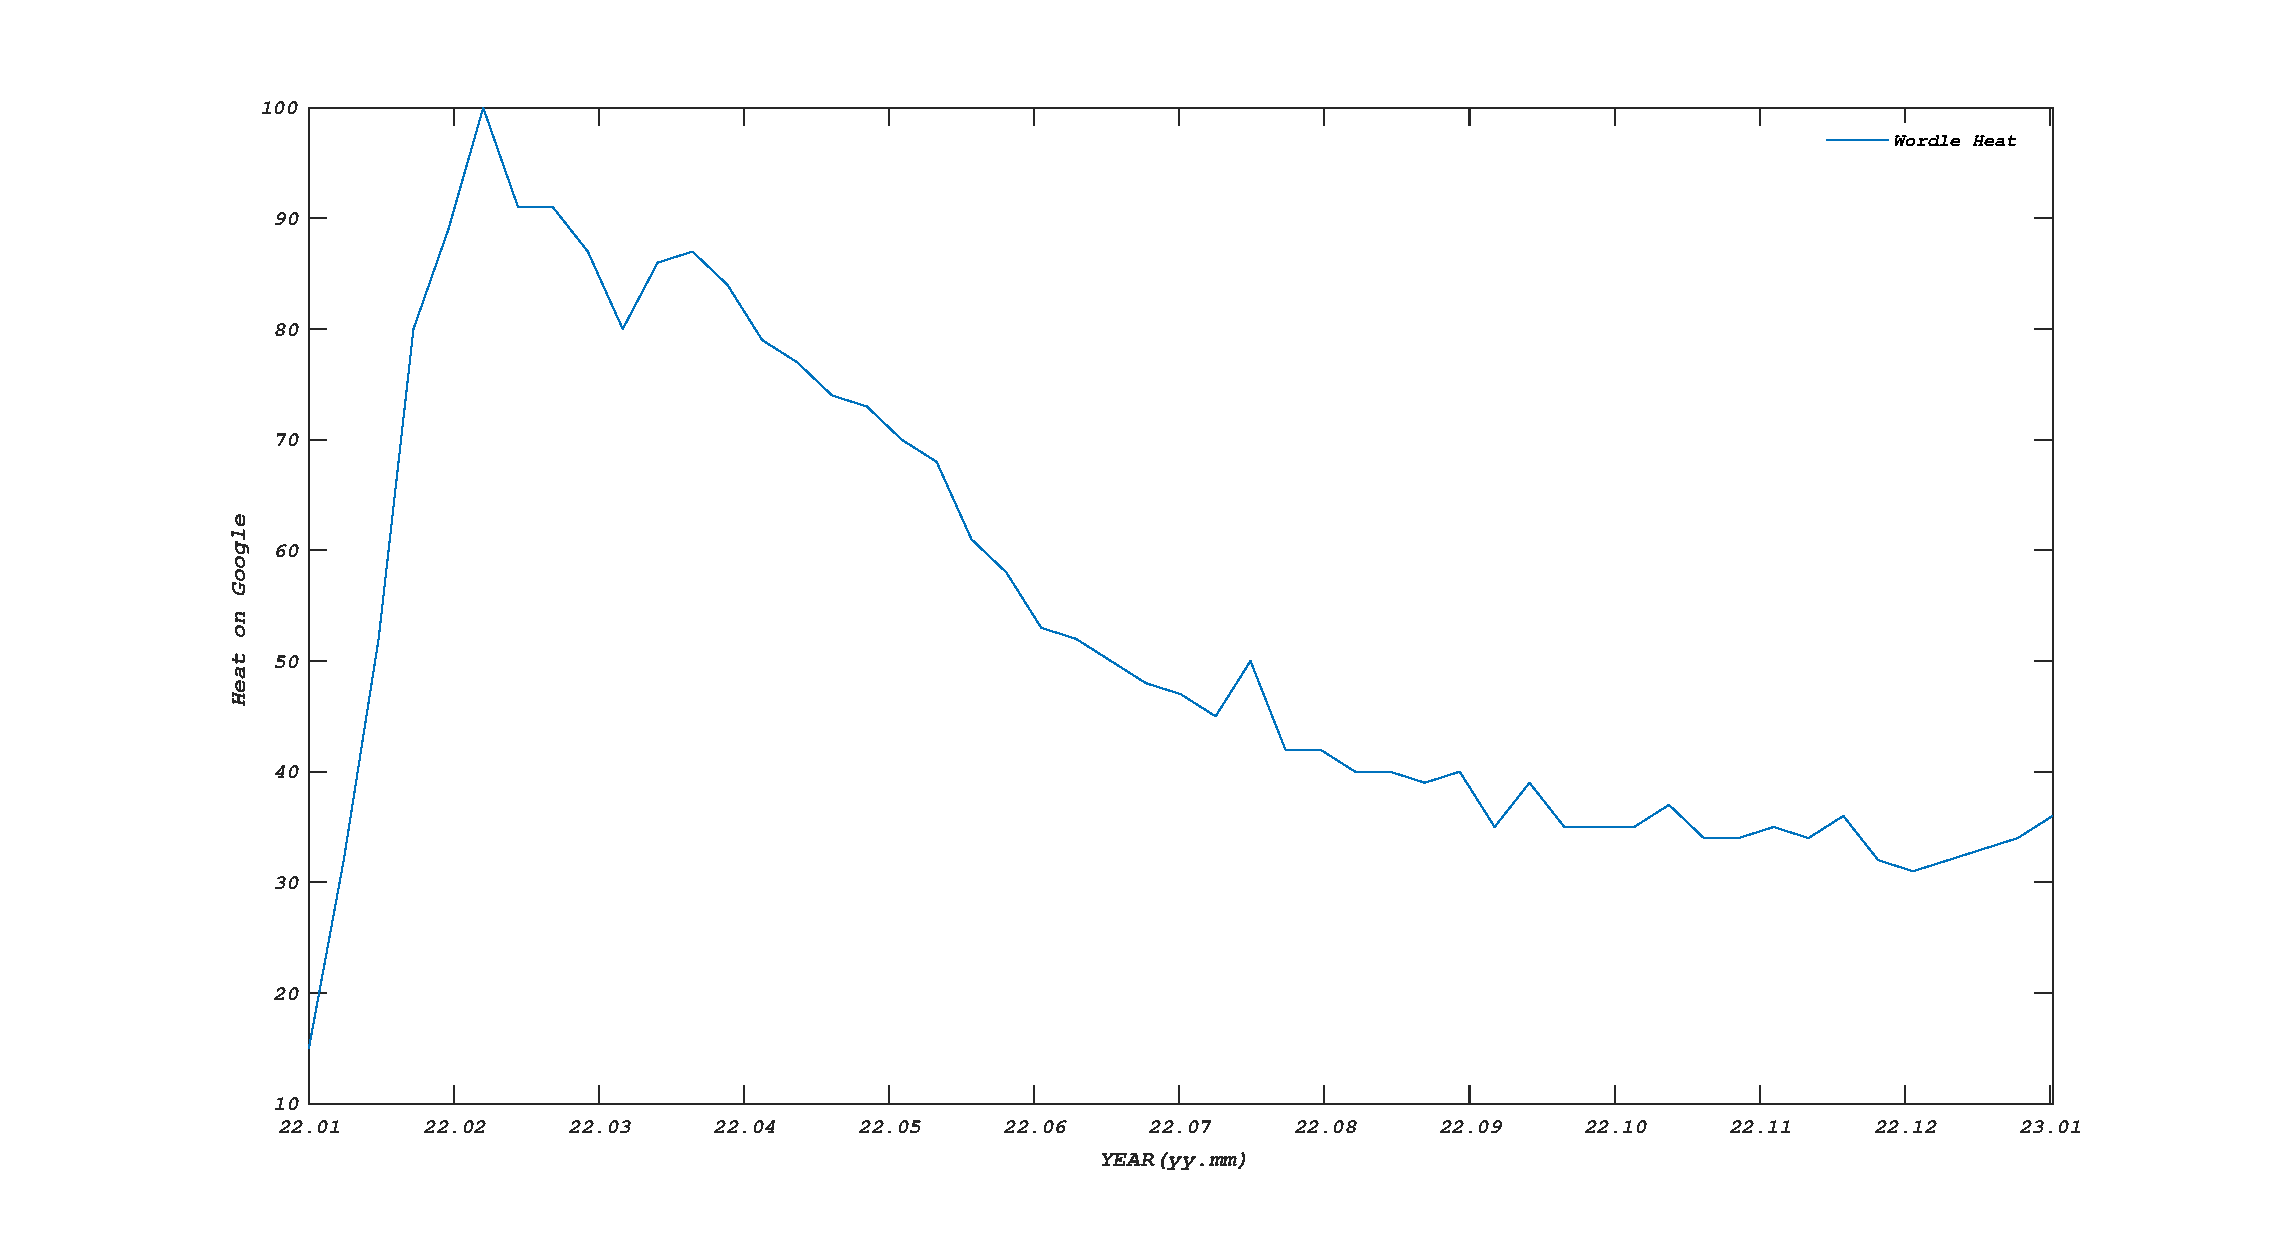
\includegraphics[width=\textwidth]{img/heat.eps}\caption{Heat on Google}
\end{subfigure}
\caption{Changing Trend of Number and Heat}\label{Changing Trend of Number and Heat}
\end{figure}
\section{Assumptions and Notations}
\subsection{Assumptions}
To simplify our model, this paper makes following basic assumption, each of which is properly
justified.
\begin{itemize}
	\item We assume that

	$\hookrightarrow$ \textbf{Justification:} Justification
\end{itemize}
\subsection{Notations}
Notations that we use in the model are shown in the Table \ref{tb:notation}:
% 三线表示例
\begin{table}[!htbp]
\begin{center}
\caption{Notations}
\begin{tabular}{clc}
	\toprule[1.5pt]
	% \multicolumn{1}{m{3cm}}
	{\centering {\itshape\textbf{Symbol}}}
	&
	% \multicolumn{1}{m{8cm}}
	{\itshape\textbf{Description}}&{\centering {\itshape\textbf{Unit}}} \\
	\midrule
	$A_i$&Level 1 indicators&- \\
	\bottomrule[1.5pt]
\end{tabular}\label{tb:notation}
\end{center}
\end{table}











\section{The Number of Reported Results}
In order to analyze and predict the number of reported results, we cleaned the data (it includes for words with incorrect number of three letters and removal of outliers from the data), and we considered the number of reports related to the Hot of the game. We represented the number of searches for ``WORDLE'' in Google as the game's hotness. They are listed in the following Figure:
\begin{figure}[htbp]
\centering
\begin{subfigure}[b]{.49\textwidth}
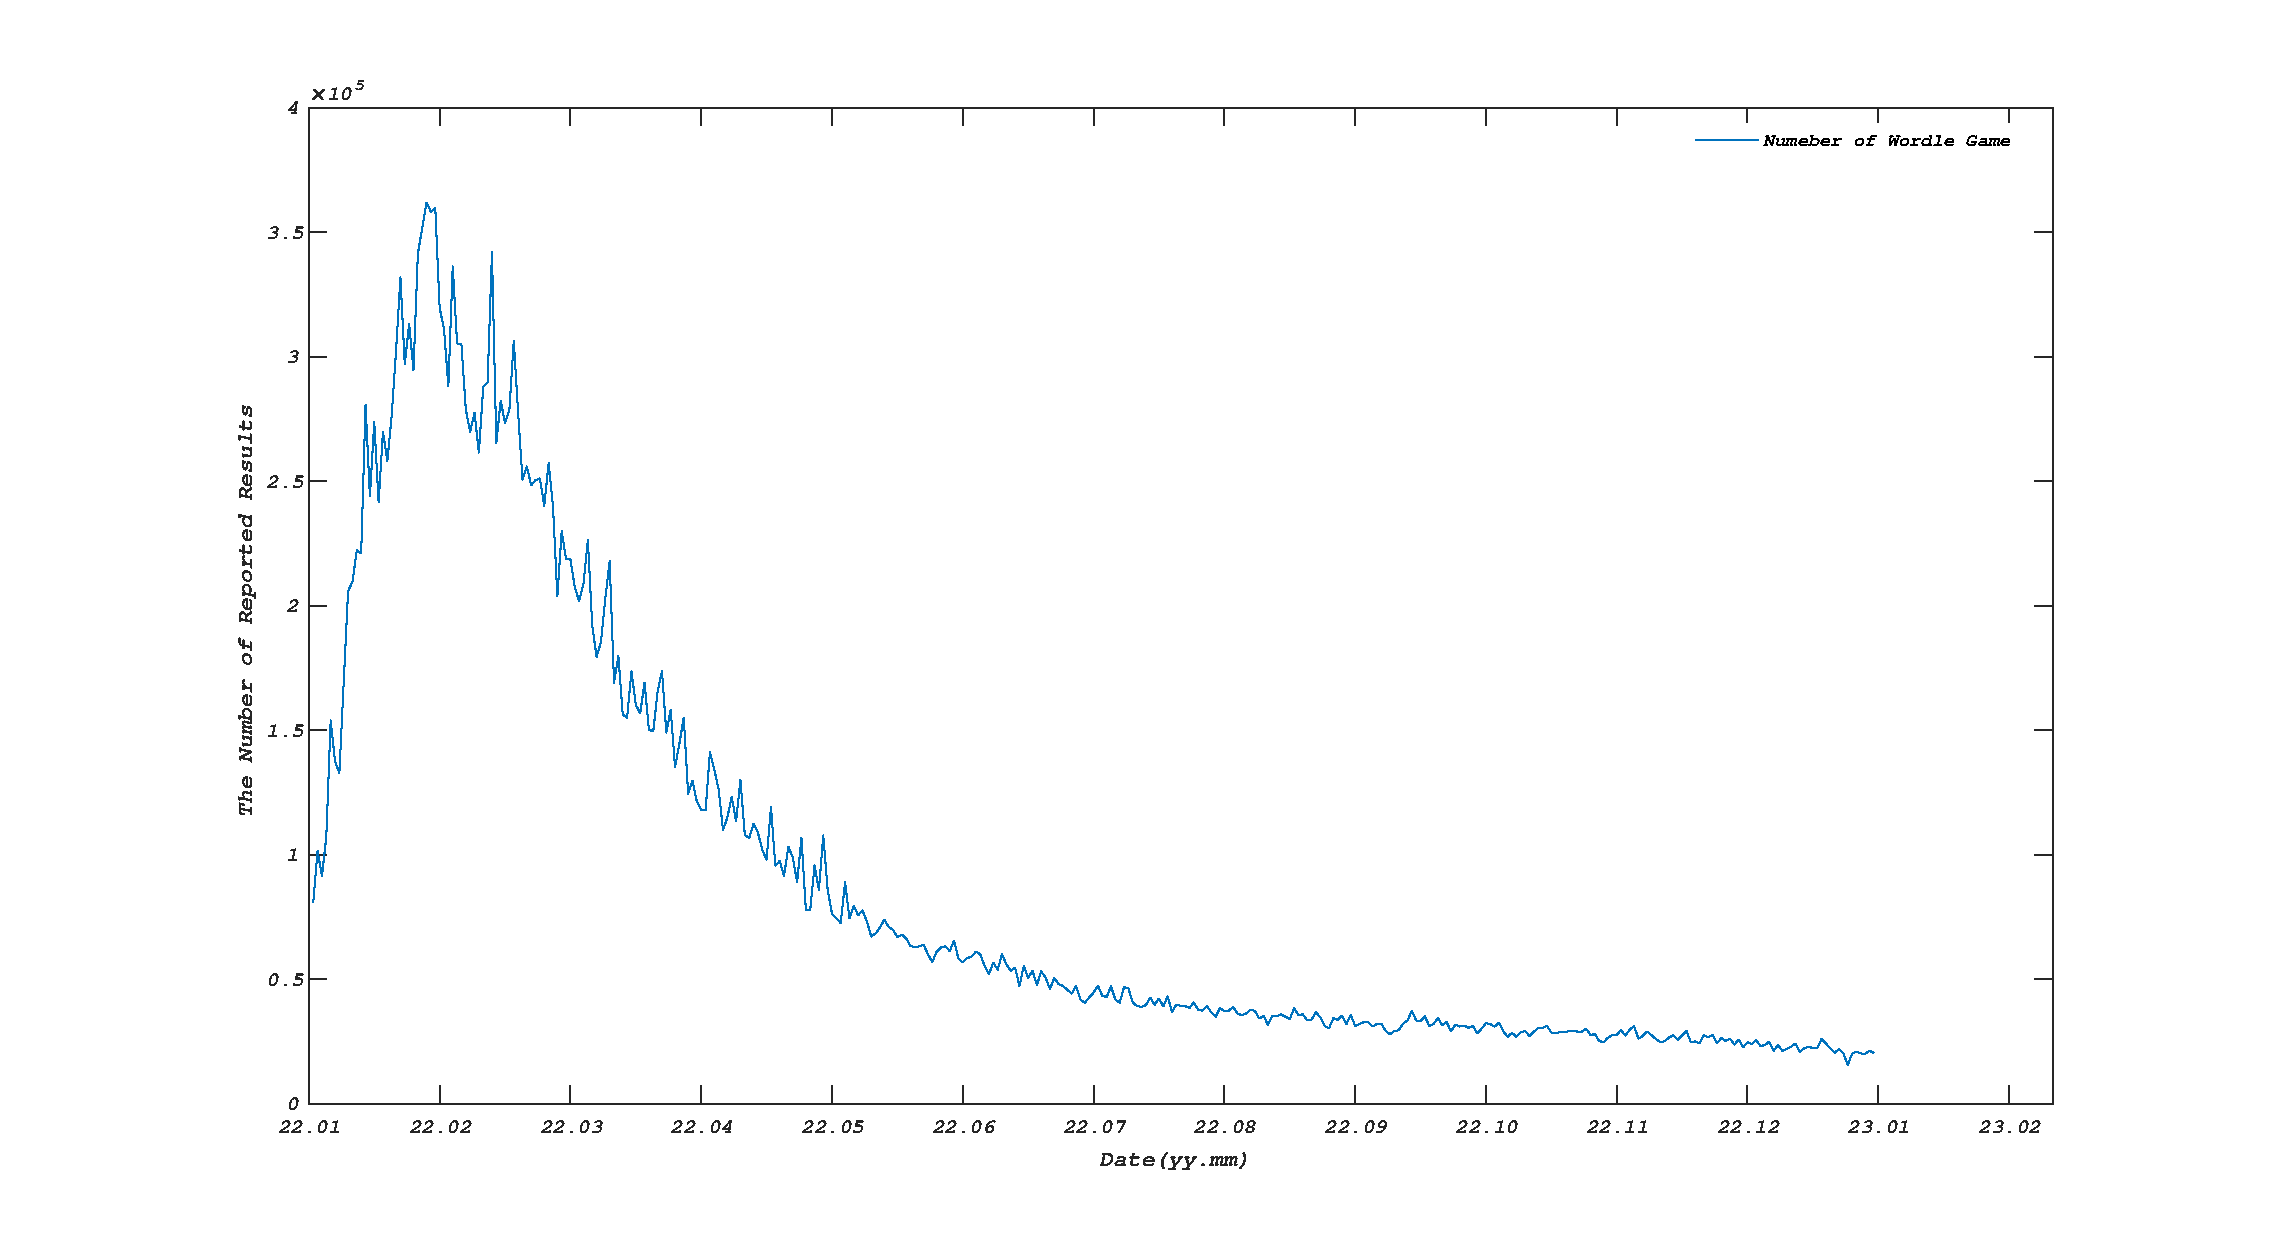
\includegraphics[width=\textwidth]{img/yuanshi.eps}\caption{The Number of Reported Results}
\end{subfigure}
\begin{subfigure}[b]{.49\textwidth}
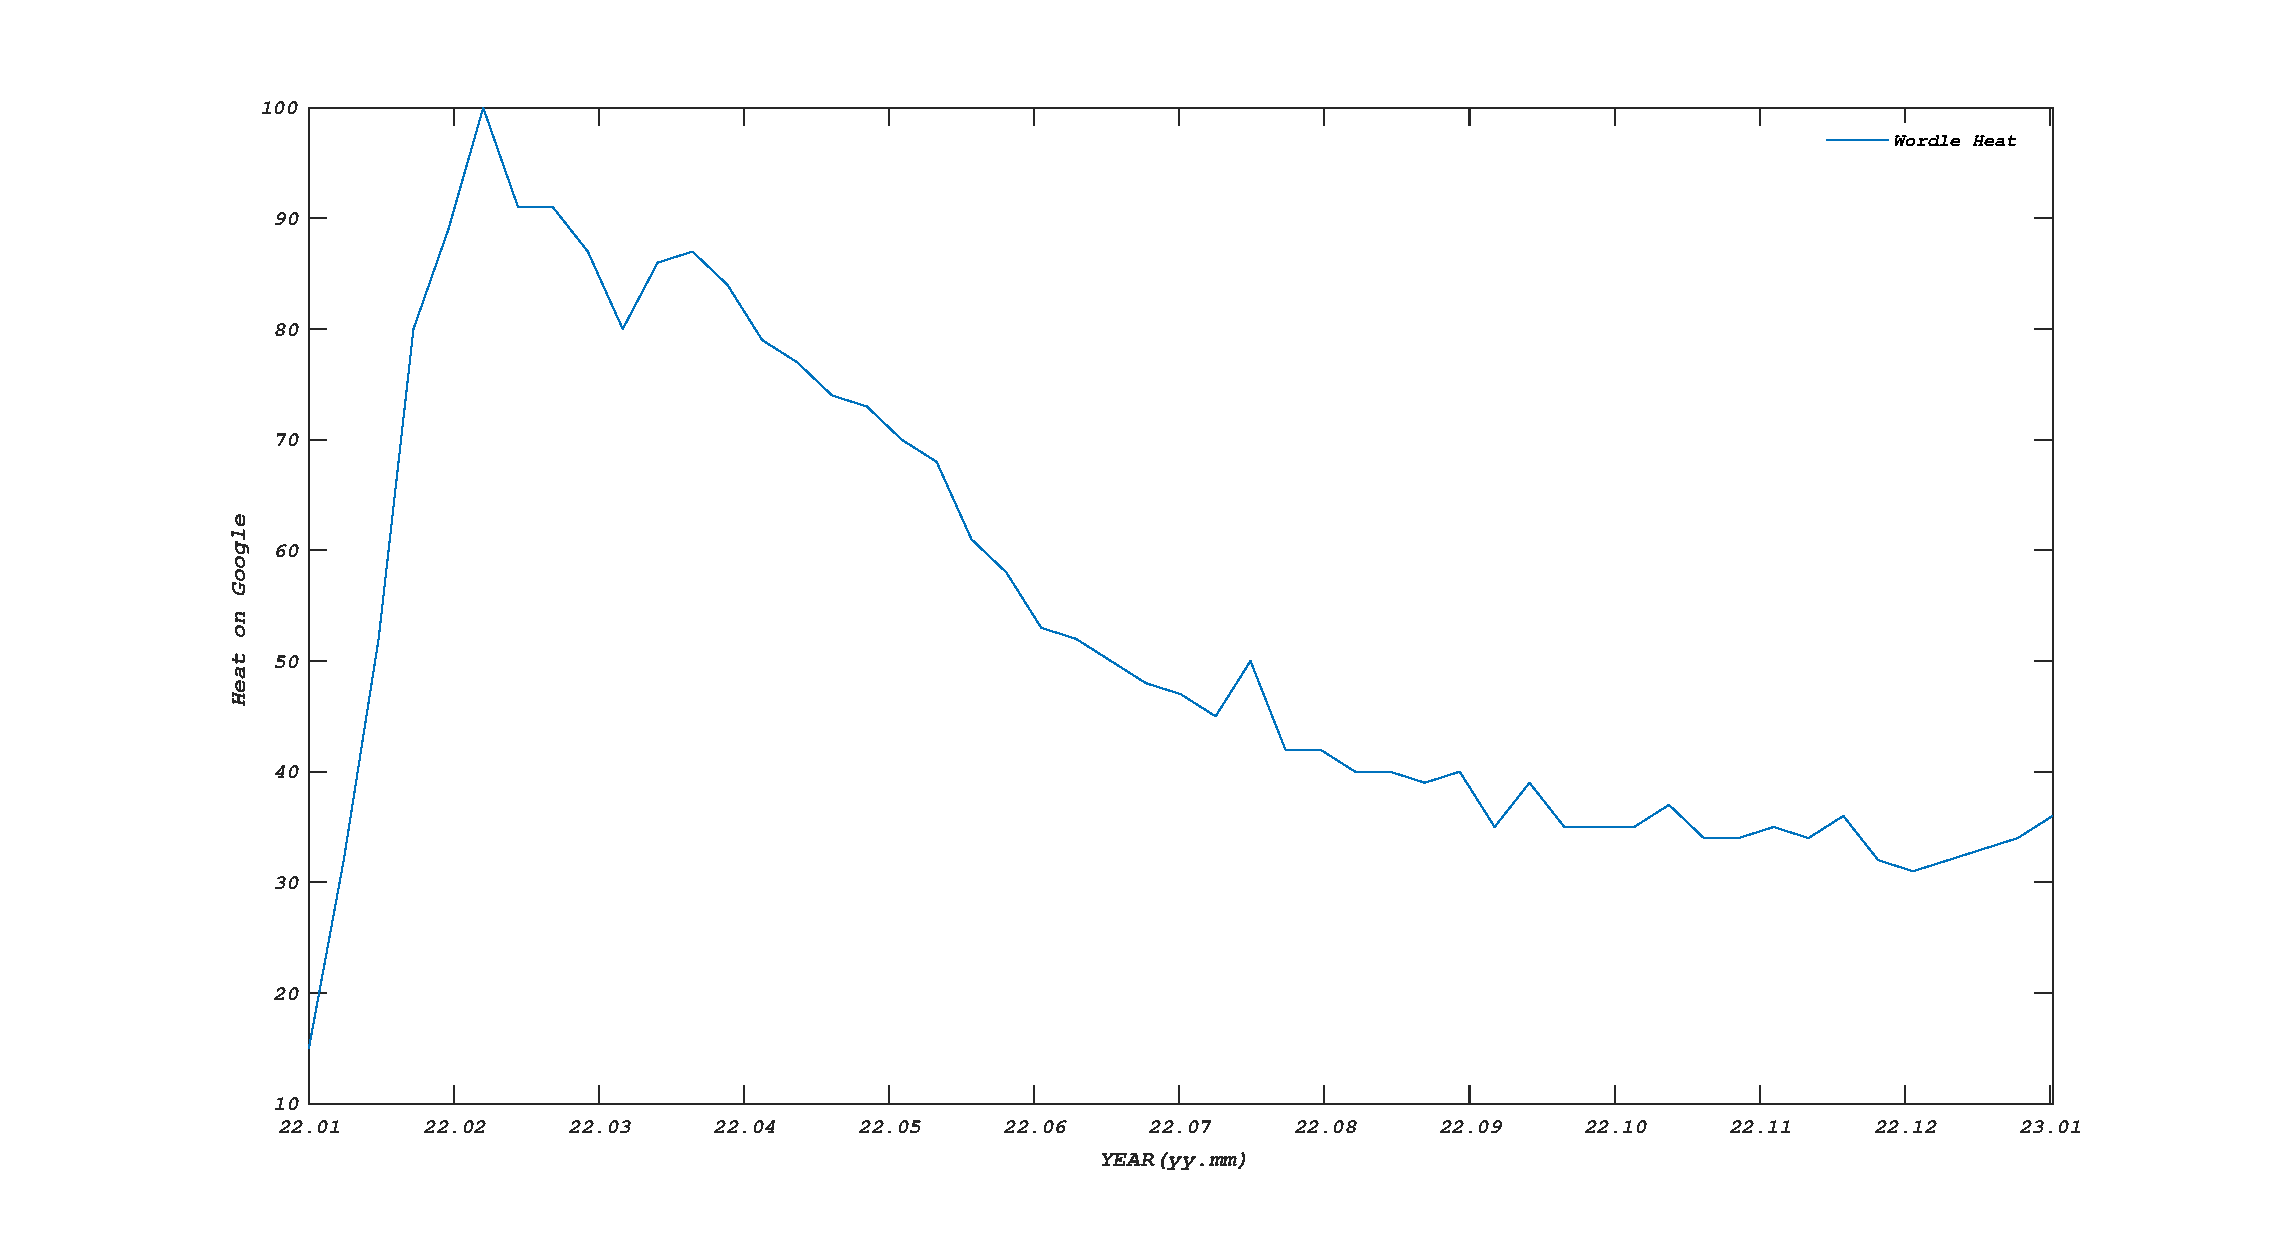
\includegraphics[width=\textwidth]{img/heat.eps}\caption{Heat on Google}
\end{subfigure}
\caption{Changing Trend of Number and Heat}\label{Changing Trend of Number and Heat}
\end{figure}

So we can easily get a preliminary conclusion: the number of reported results changes with the change in the heat of ``WORDLE'' on Google, and there is a positive correlation between the two before. We this explains the reason for the change in the number of reported results: because of the change in the heat of the game. Of course this is only a simple model, in order to get a concrete picture of how the number of reports changes and how the number of reports will change in the future, we will build a mathematical model below and get the number of reports in the interval of March 1, 2023.
\subsection{Establishment of ARIMA Model}
\subsubsection{ARIMA Model Introduction}
The Autoregressive Integrated Moving Average model (\textbf{ARIMA}) is a type of time series forecasting model that allows us to transform our non-stationary time series into a stationary time series after finite difference processing. ARIMA is the most common in the series family due to the adaptability of linear patterns amongst
all time series strategies. Moreover, ARIMA model has the benefits of using a simpler algorithm and being
a studied technology in comparison to the second generation of forecasting methods which is the artificial neural
networks.
\subsubsection{Mathematical Modeling of ARIMA}
The mathematical model of ARIMA ($p, d, q$) is shown to be precise in the literature by combining AR ($p$)
and MA ($q$), While Integrated (\textbf{I}) reflects the separation of raw observations to allow the time series to become
stationary, the difference between the real data values, and the previous values are replaced with the data values.
The finite distinction of the data points in ARIMA ($p, d, q$) are used to transform the non-stationary time series to
the steady one. The mathematical formulation of ARIMA ($p, d, q$) is demonstrated as following Equations.
\begin{eqnarray}
	\varphi (L)(1-L)^dy_t & = & \theta (L)\varepsilon _t
\end{eqnarray}
\begin{eqnarray}
	(1-\sum_{i=0}^{p}\varphi _iL^i)(1-L)^dy_t=(1+\sum_{j=1}^q\theta_jL^j)\varepsilon_t
\end{eqnarray}
\begin{eqnarray}
	Y_t=\phi _0+\phi_1y_{t-1}+\phi_2y_{t-2}+\cdots +\phi_py_{t-p}+\varepsilon _t-\theta_1\varepsilon_{t-1}-\theta_2\varepsilon_{t-2}-\cdots-\theta_p\varepsilon_{t-p}
\end{eqnarray}
Where $y_t$ and $\varepsilon_t$ are the actual value and random error at time period $t$,respectively.$\varphi_1(i=1,2,\cdots ,p)$ and $\theta_j(j=0,1,\cdots ,q)$ are model paramenters. $p,d$ and $q$ are positive integers, referring to the order of the autoregressive, integrated, and moving average parts of the model, respectively. A typical method for identifying $p$ and $q$ is achieved by implementation of the Autocorrelation Function (\textbf{ACF}) and Partial Autocorrelation Functions (\textbf{PACF}) of the data.
The PACF plot helps to decide if the ACF plot can classify non-stationary time series by the maximum order of
AR ($p$).
\subsection{Solution of ARIMA Model}
We will use matlab and the above model to explain and predict the changes in the number of reports as follows:
\subsubsection{Determination of $d$}
Before the ARIMA model, we first have to perform a smoothness test on the time series. And we use matlab to perform the smoothness test to find that the series is not smooth, after the first order difference, the time series is smooth, so we get $d=1$.
\subsubsection{Determination of $p,q$}
There is no good way to determine $p$ and $q$, but the computer is obviously better than the naked eye for $p,q$. We select the better ARIMA model by a series of variations of $p,q$ values.
\subsubsection{Model Selection}
For the selection of the ARIMA model, we found the better set, which obtained the $Adjusted-R^2, AIC, SC, MAPE$ and $RMSE$ we shown it in Table \ref{r2}:
\begin{table}[]
\centering
\caption{Test Index of Each Model}\label{r2}
\resizebox{\textwidth}{!}{
\begin{tabular}{ccccccc}
\hline
\textbf{Index} &
  \textbf{ARIMA (1,1,0)} &
  \textbf{ARIMA (2,1,0)} &
  \textbf{ARIMA (3,1,0)} &
  \textbf{ARIMA (2,1,0)} &
  \textbf{ARIMA (5,1,0)} &
  \textbf{ARIMA (6,1,0)} \\ 
\textbf{Adjusted-R$^2$} &
  0.351697 &
  0.352447 &
  0.139293 &
  0.311184 &
  0.394786 &
  0.279782 \\
\textbf{AIC} &
  7.514608 &
  7.513726 &
  7.784217 &
  7.573689 &
  7.449272 &
  7.696297 \\
\textbf{SC} &
  7.627180 &
  7.626297 &
  7.896789 &
  7.686260 &
  7.561843 &
  7.808869 \\
\textbf{MAPE} &
  6.576058 &
  6.573973 &
  8.285324 &
  6.847210 &
  5.991413 &
  6.680915 \\
\textbf{RMSE} &
  9.717137 &
  9.713131 &
  11.16802 &
  10.01724 &
  9.454456 &
  10.66723 \\ \hline
\textbf{Index} &
  \textbf{ARIMA (1,1,1)} &
  \textbf{ARIMA (2,1,1)} &
  \textbf{ARIMA (3,1,1)} &
  \textbf{ARIMA (4,1,1)} &
  \textbf{ARIMA (5,1,1)} &
  \textbf{ARIMA (6,1,1)} \\
\textbf{Adjusted-R$^2$} &
  0.282660 &
  0.302913 &
  0.224594 &
  0.094755 &
  0.282594 &
  0.144170 \\
\textbf{AIC} &
  7.505304 &
  7.487031 &
  7.574546 &
  7.898818 &
  7.505778 &
  7.703474 \\
\textbf{SC} &
  7.622254 &
  7.603981 &
  7.691496 &
  8.011390 &
  7.622728 &
  7.820424 \\
\textbf{MAPE} &
  5.495101 &
  5.439750 &
  5.682568 &
  8.502531 &
  5.430309 &
  6.579909 \\
\textbf{RMSE} &
  9.637975 &
  9.514886 &
  10.00691 &
  11.98773 &
  9.725911 &
  10.72635 \\ \hline
\textbf{Index} &
  \textbf{ARIMA (1,1,2)} &
  \textbf{ARIMA (2,1,2)} &
  \textbf{ARIMA (3,1,2)} &
  \multicolumn{1}{c}{\textbf{ARIMA (4,1,2)}} &
  {\color[HTML]{000000} \textbf{ARIMA (5,1,2)}} &
  \textbf{ARIMA (6,1,2)} \\
\textbf{Adjusted-R$^2$} &
  0.066860 &
  0.151594 &
  0.356335 &
  \multicolumn{1}{c}{0.001429} &
  \multicolumn{1}{c}{{\color[HTML]{CB0000} \textit{\textbf{0.401740}}}} &
  0.151327 \\
\textbf{AIC} &
  7.869510 &
  7.776217 &
  7.507592 &
  \multicolumn{1}{c}{7.928901} &
  \multicolumn{1}{c}{{\color[HTML]{CB0000} \textit{\textbf{7.373051}}}} &
  7.779057 \\
\textbf{SC} &
  7.982082 &
  7.888789 &
  7.620164 &
  \multicolumn{1}{c}{8.041473} &
  \multicolumn{1}{c}{{\color[HTML]{CB0000} \textit{\textbf{7.490001}}}} &
  7.891629 \\
\textbf{MAPE} &
  7.673681 &
  7.285152 &
  6.719789 &
  \multicolumn{1}{c}{8.376965} &
  \multicolumn{1}{c}{{\color[HTML]{CB0000} \textit{\textbf{5.072340}}}} &
  7.482382 \\
\textbf{RMSE} &
  11.68773 &
  11.14531 &
  9.854205 &
  \multicolumn{1}{c}{12.19098} &
  \multicolumn{1}{c}{{\color[HTML]{CB0000} \textit{\textbf{8.884206}}}} &
  11.26219 \\ \hline
\textbf{Index} &
  \textbf{ARIMA (1,1,3)} &
  \textbf{ARIMA (2,1,3)} &
  \textbf{ARIMA (3,1,3)} &
  \textbf{ARIMA (4,1,3)} &
  \textbf{ARIMA (5,1,3)} &
  \textbf{ARIMA (6,1,3)} \\
\textbf{Adjusted-R$^2$} &
  0.013991 &
  0.207111 &
  0.292092 &
  0.123519 &
  -0.015869 &
  0.149244 \\
\textbf{AIC} &
  7.814235 &
  7.635996 &
  7.493233 &
  7.721904 &
  7.841370 &
  7.692927 \\
\textbf{SC} &
  7.931185 &
  7.752946 &
  7.610183 &
  7.838854 &
  7.958320 &
  7.809877 \\
\textbf{MAPE} &
  6.998548 &
  6.020232 &
  5.687182 &
  6.844513 &
  7.251816 &
  6.197987 \\
\textbf{RMSE} &
  11.41146 &
  10.29992 &
  9.765165 &
  10.89394 &
  11.70910 &
  10.75731 \\ \hline
\end{tabular}}
\end{table}
\subsection{Prediction of March 1, 2023}
We chose ARIMA(5,1,2) as our final ARIMA model by which we forecast the March 1, 2023 quantity. And give the forecast interval based on the model error:$\bm{[30943,33839]}$.
\begin{figure}[htbp]
\centering
\begin{subfigure}[b]{.49\textwidth}
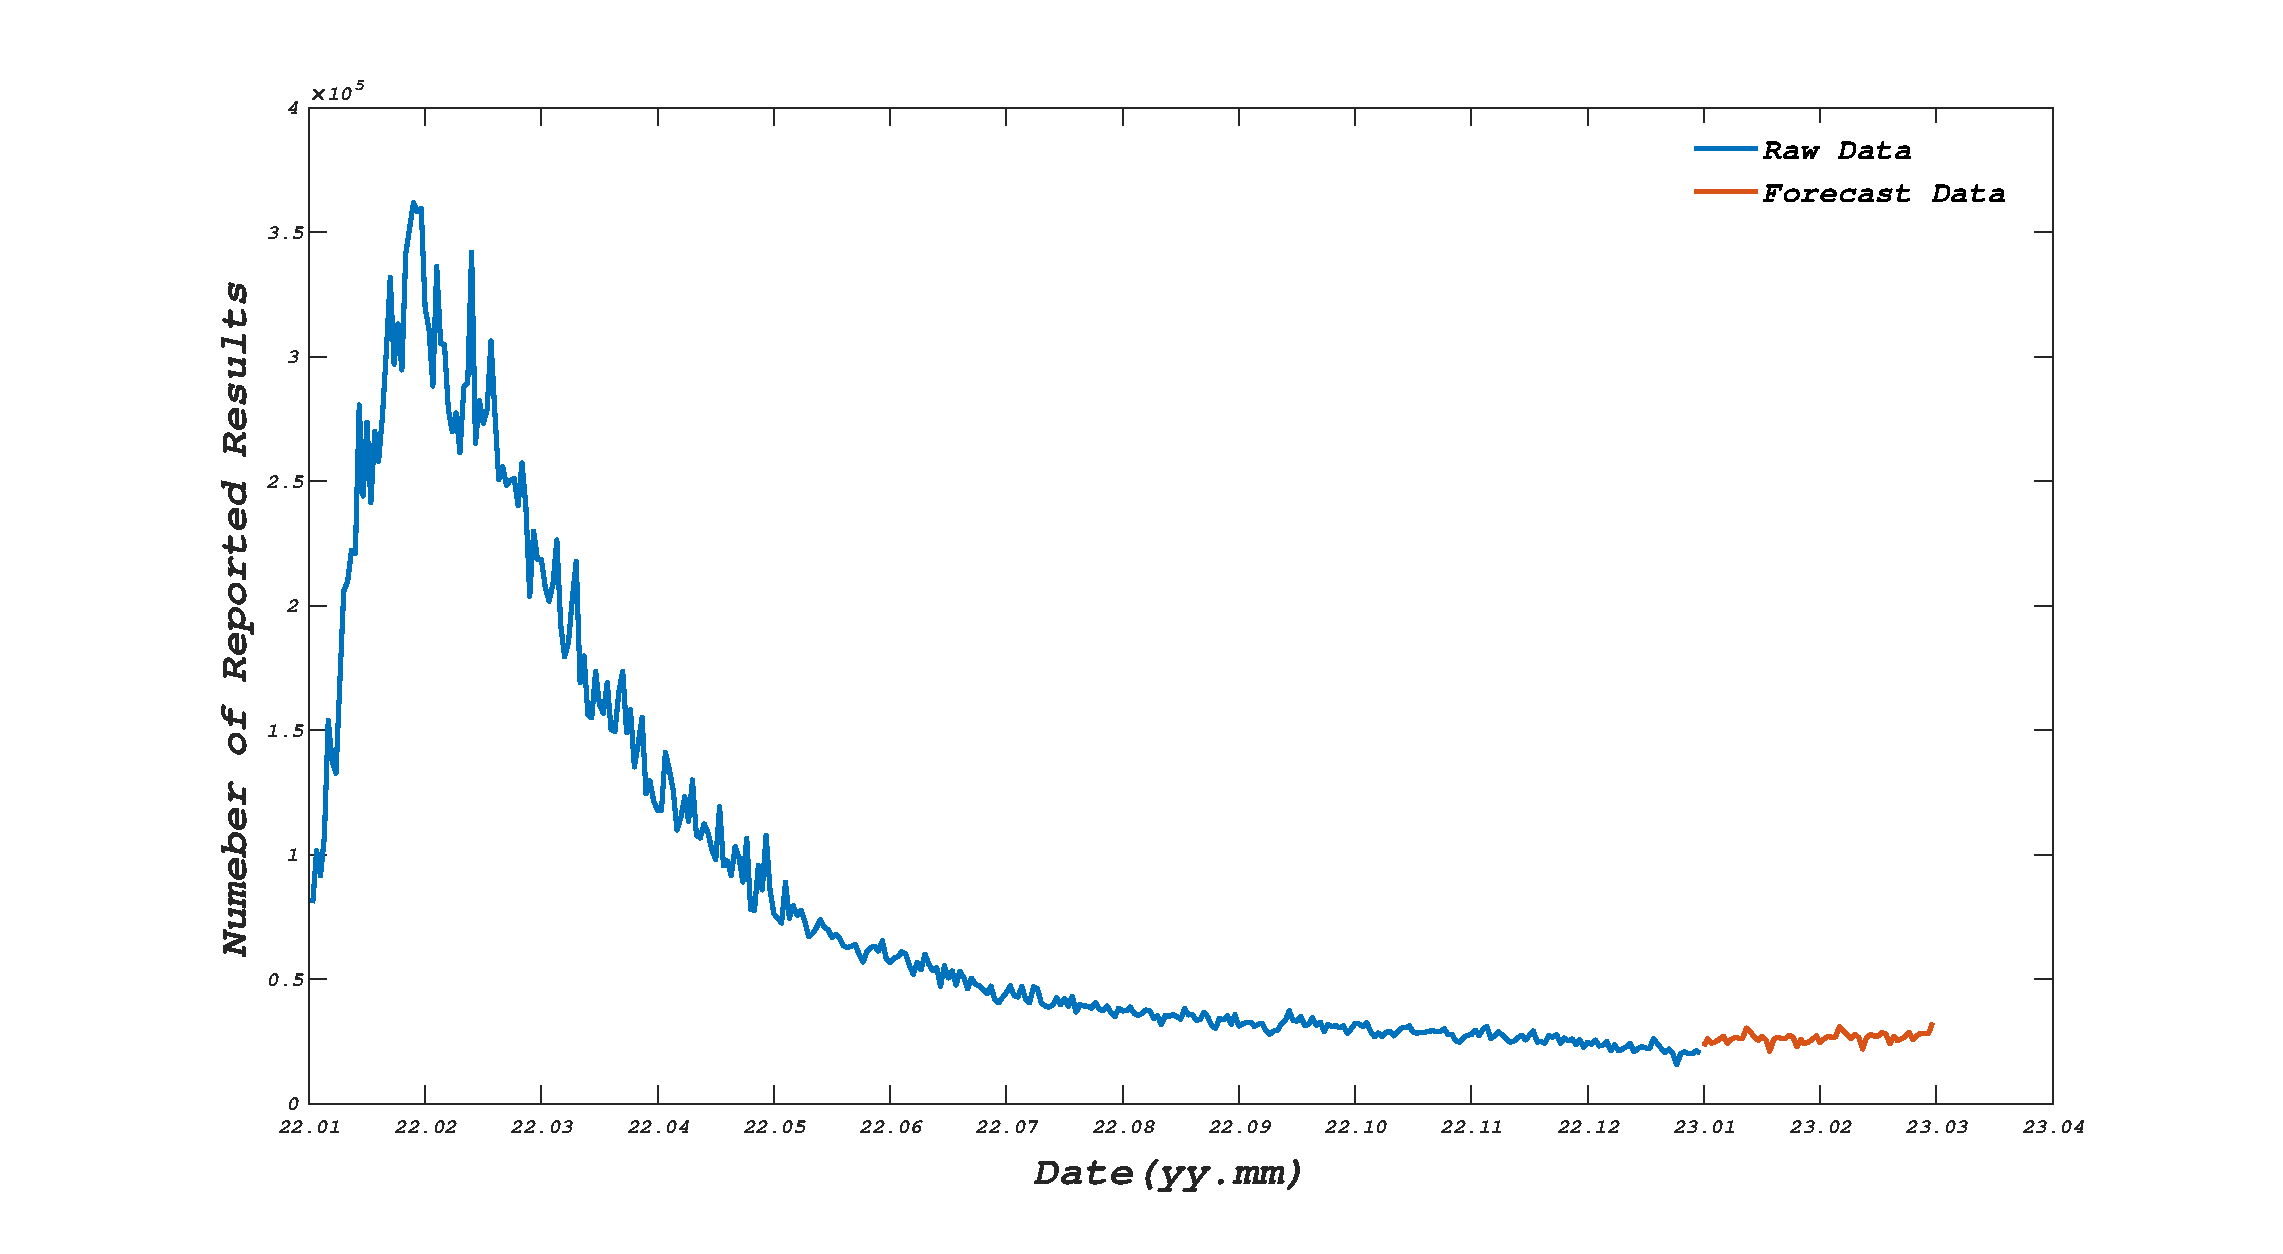
\includegraphics[width=\textwidth]{img/yuce.eps}\caption{Prediction Results}
\end{subfigure}
\begin{subfigure}[b]{.49\textwidth}
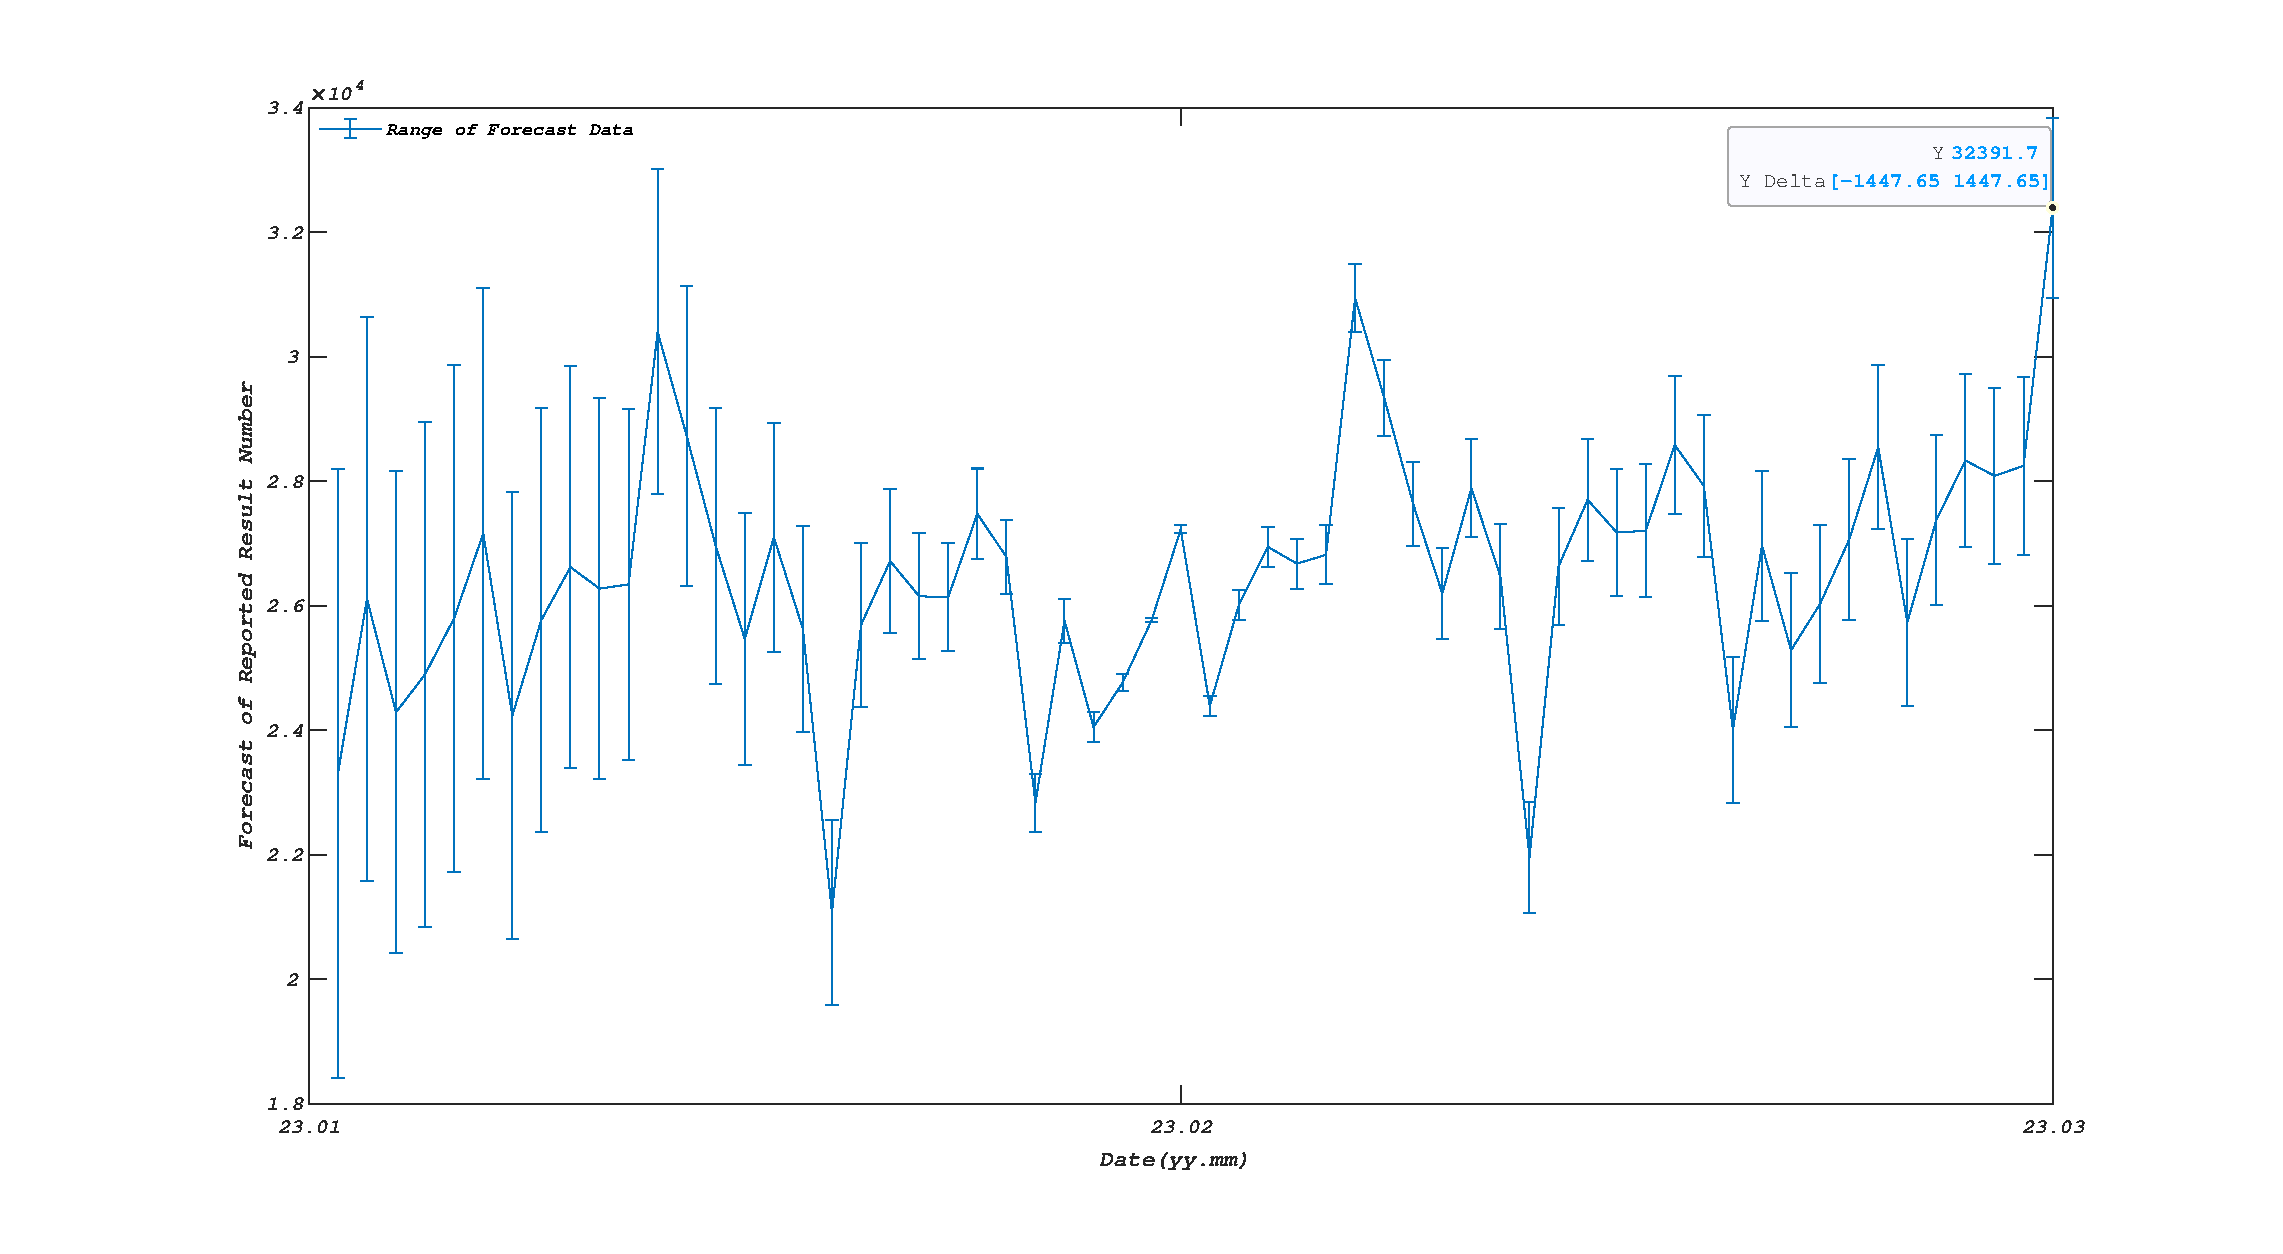
\includegraphics[width=\textwidth]{img/wucha.eps}\caption{Prediction Interval}
\end{subfigure}
\caption{ARIMA(5,1,2) Model Predict}
\end{figure}
\begin{figure}[htbp]
\centering
\begin{subfigure}[b]{.49\textwidth}
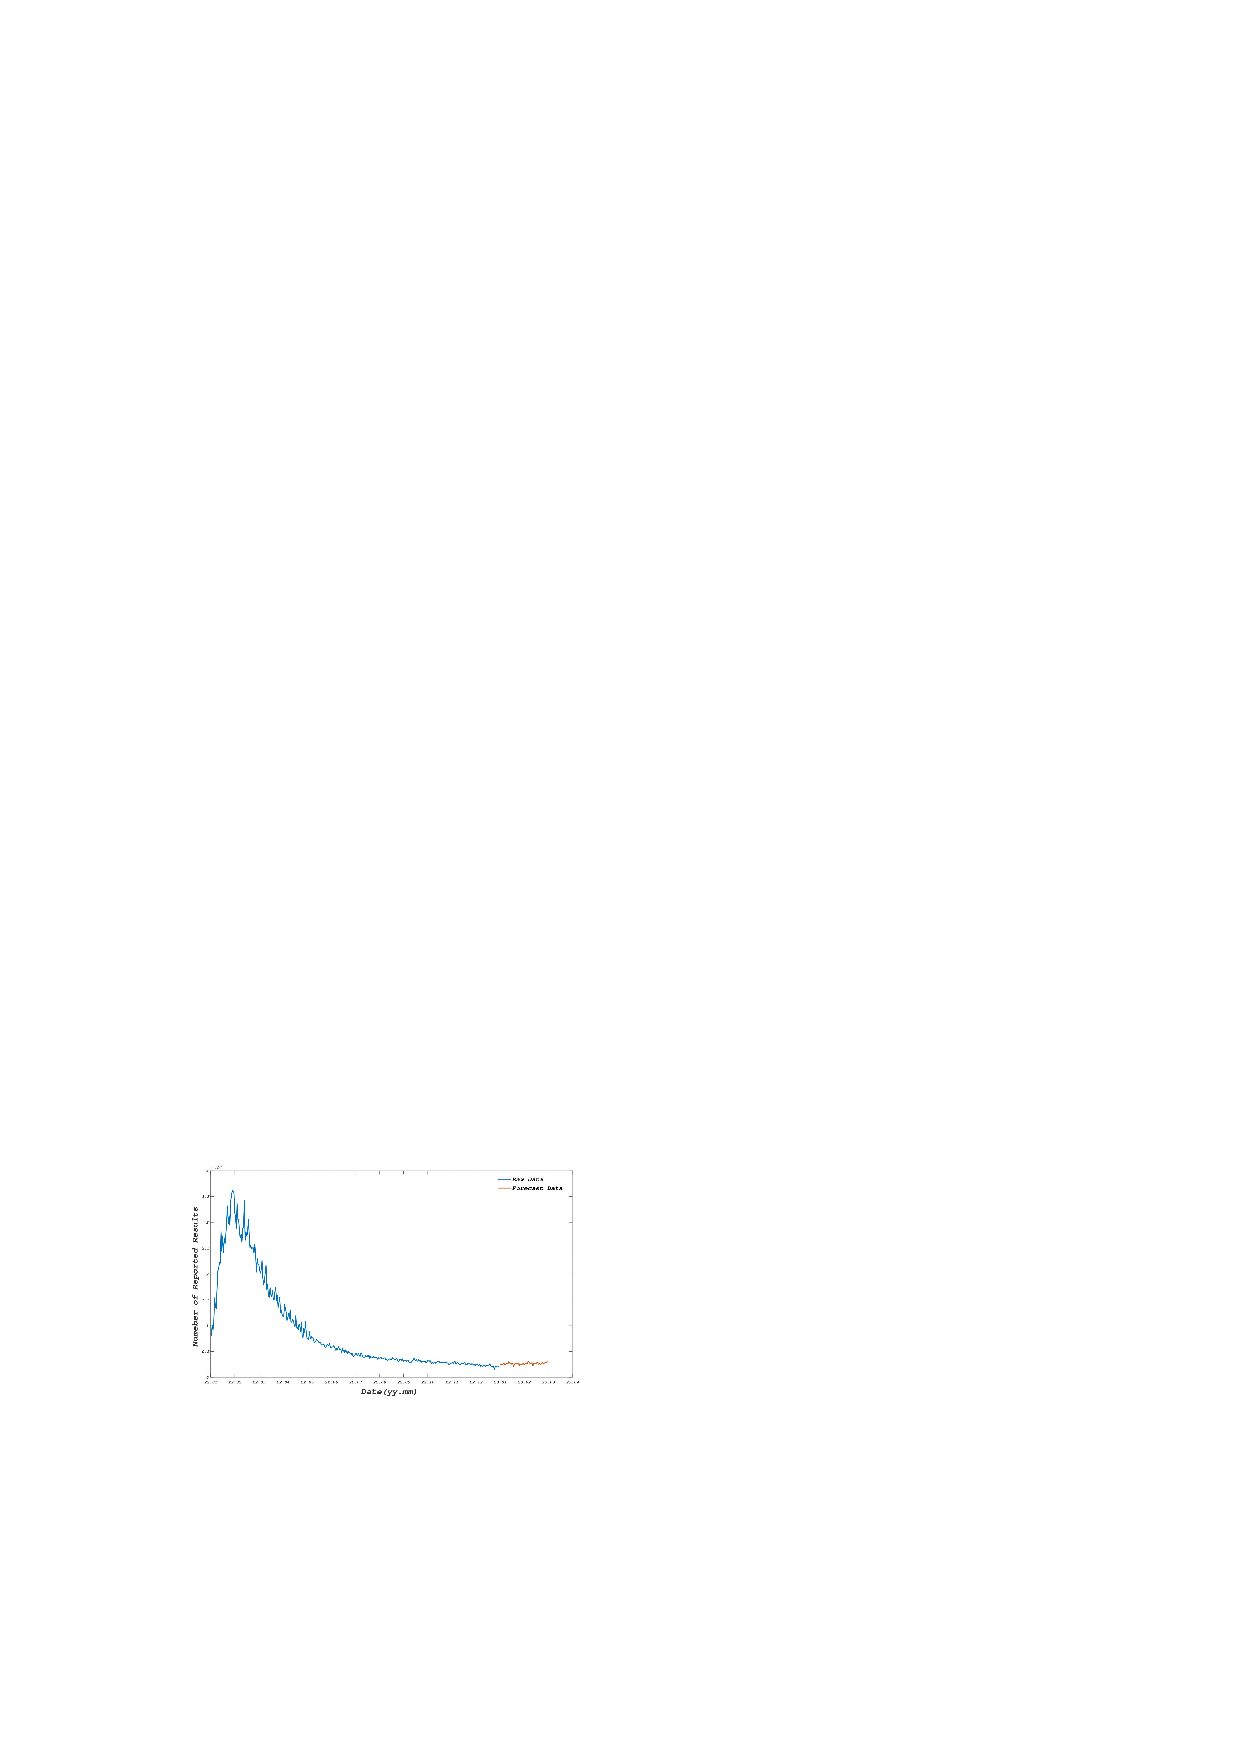
\includegraphics[width=\textwidth]{img/yuanshi.pdf}\caption{Prediction Results}
\end{subfigure}
\begin{subfigure}[b]{.49\textwidth}
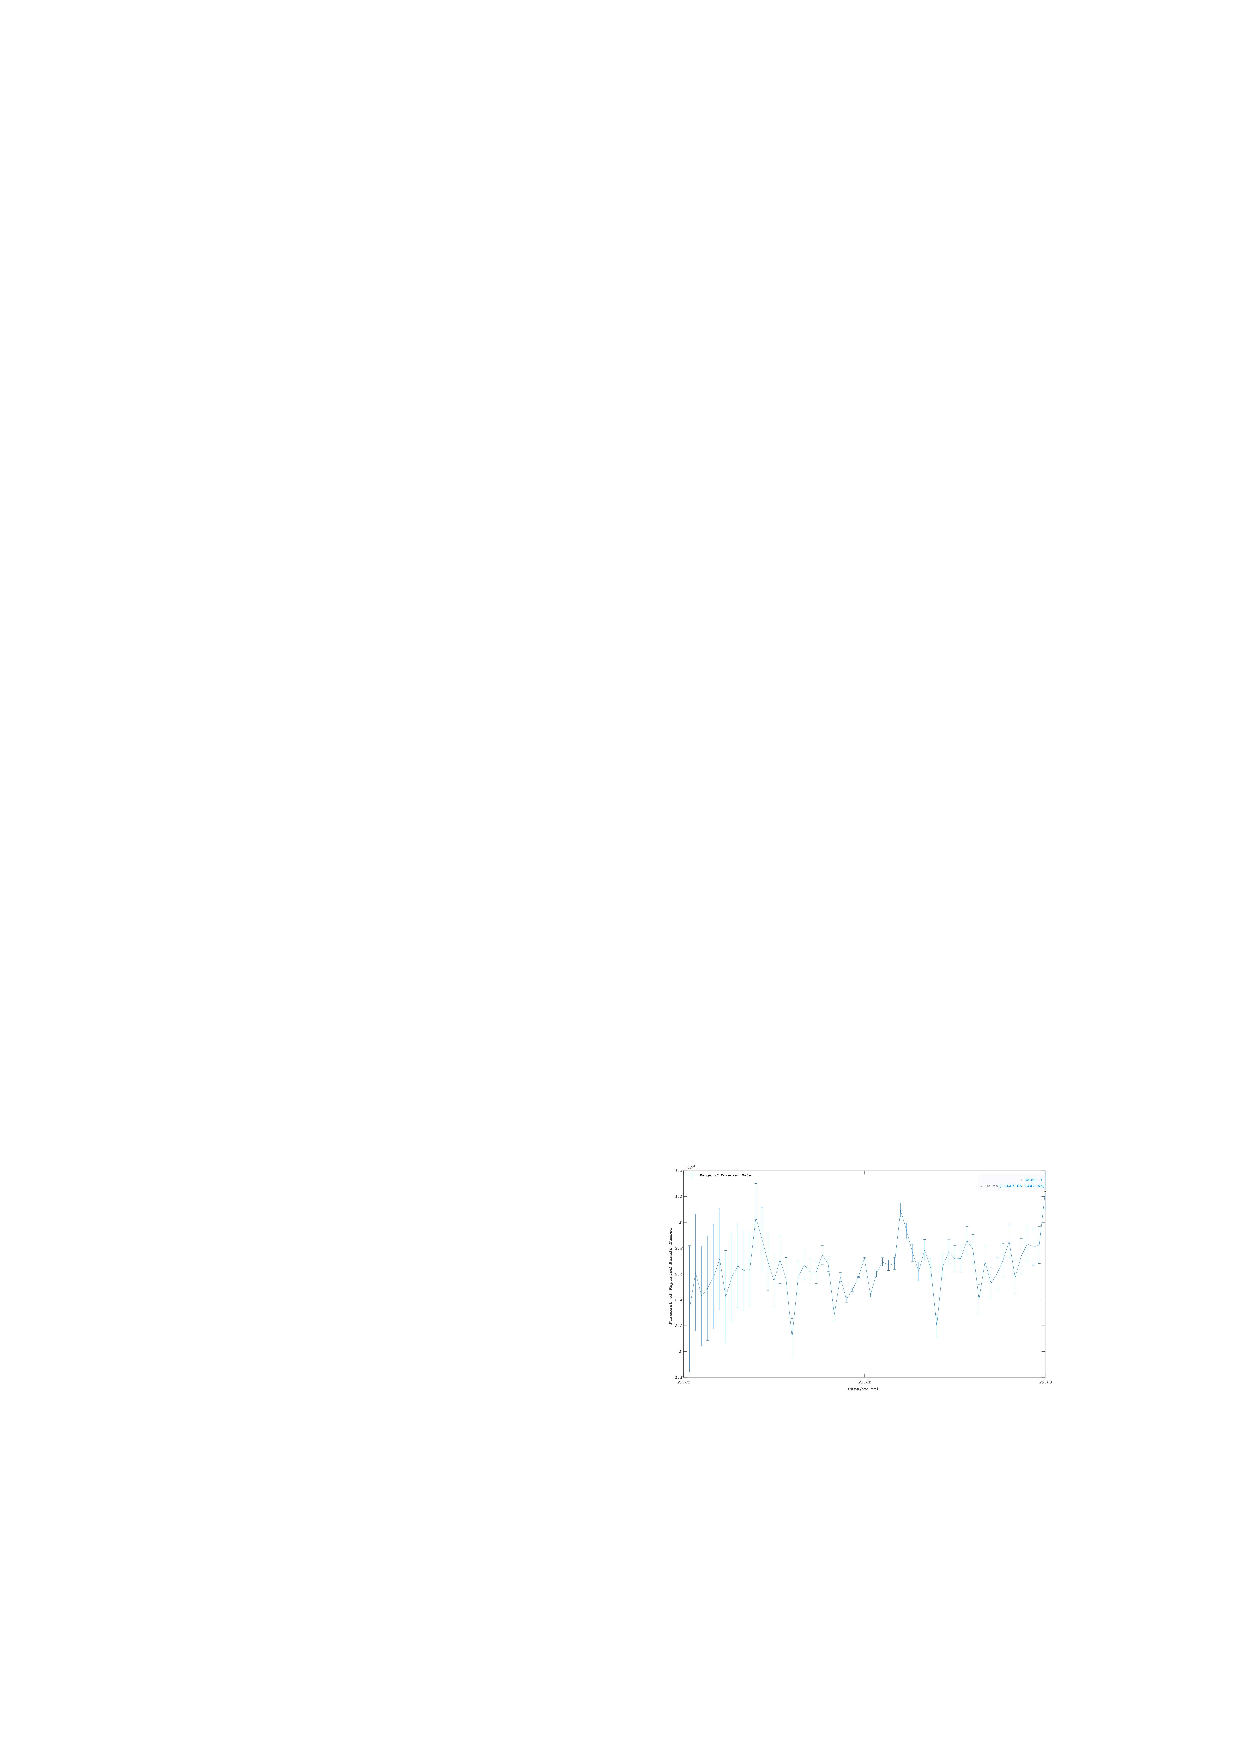
\includegraphics[width=\textwidth]{img/wucha.pdf}\caption{Prediction Interval}
\end{subfigure}
\caption{ARIMA(5,1,2) Model Predict}
\end{figure}










































\subsection{Model I}

\begin{enumerate}
    \renewcommand{\labelenumi}{\textbf{Step \theenumi}}
    \item 

\end{enumerate}



































































\section{Solution For Problem One}
% \subsection{subsection}
% \begin{figure}[htbp]
% \centering
% \begin{subfigure}[b]{.32\textwidth}
% 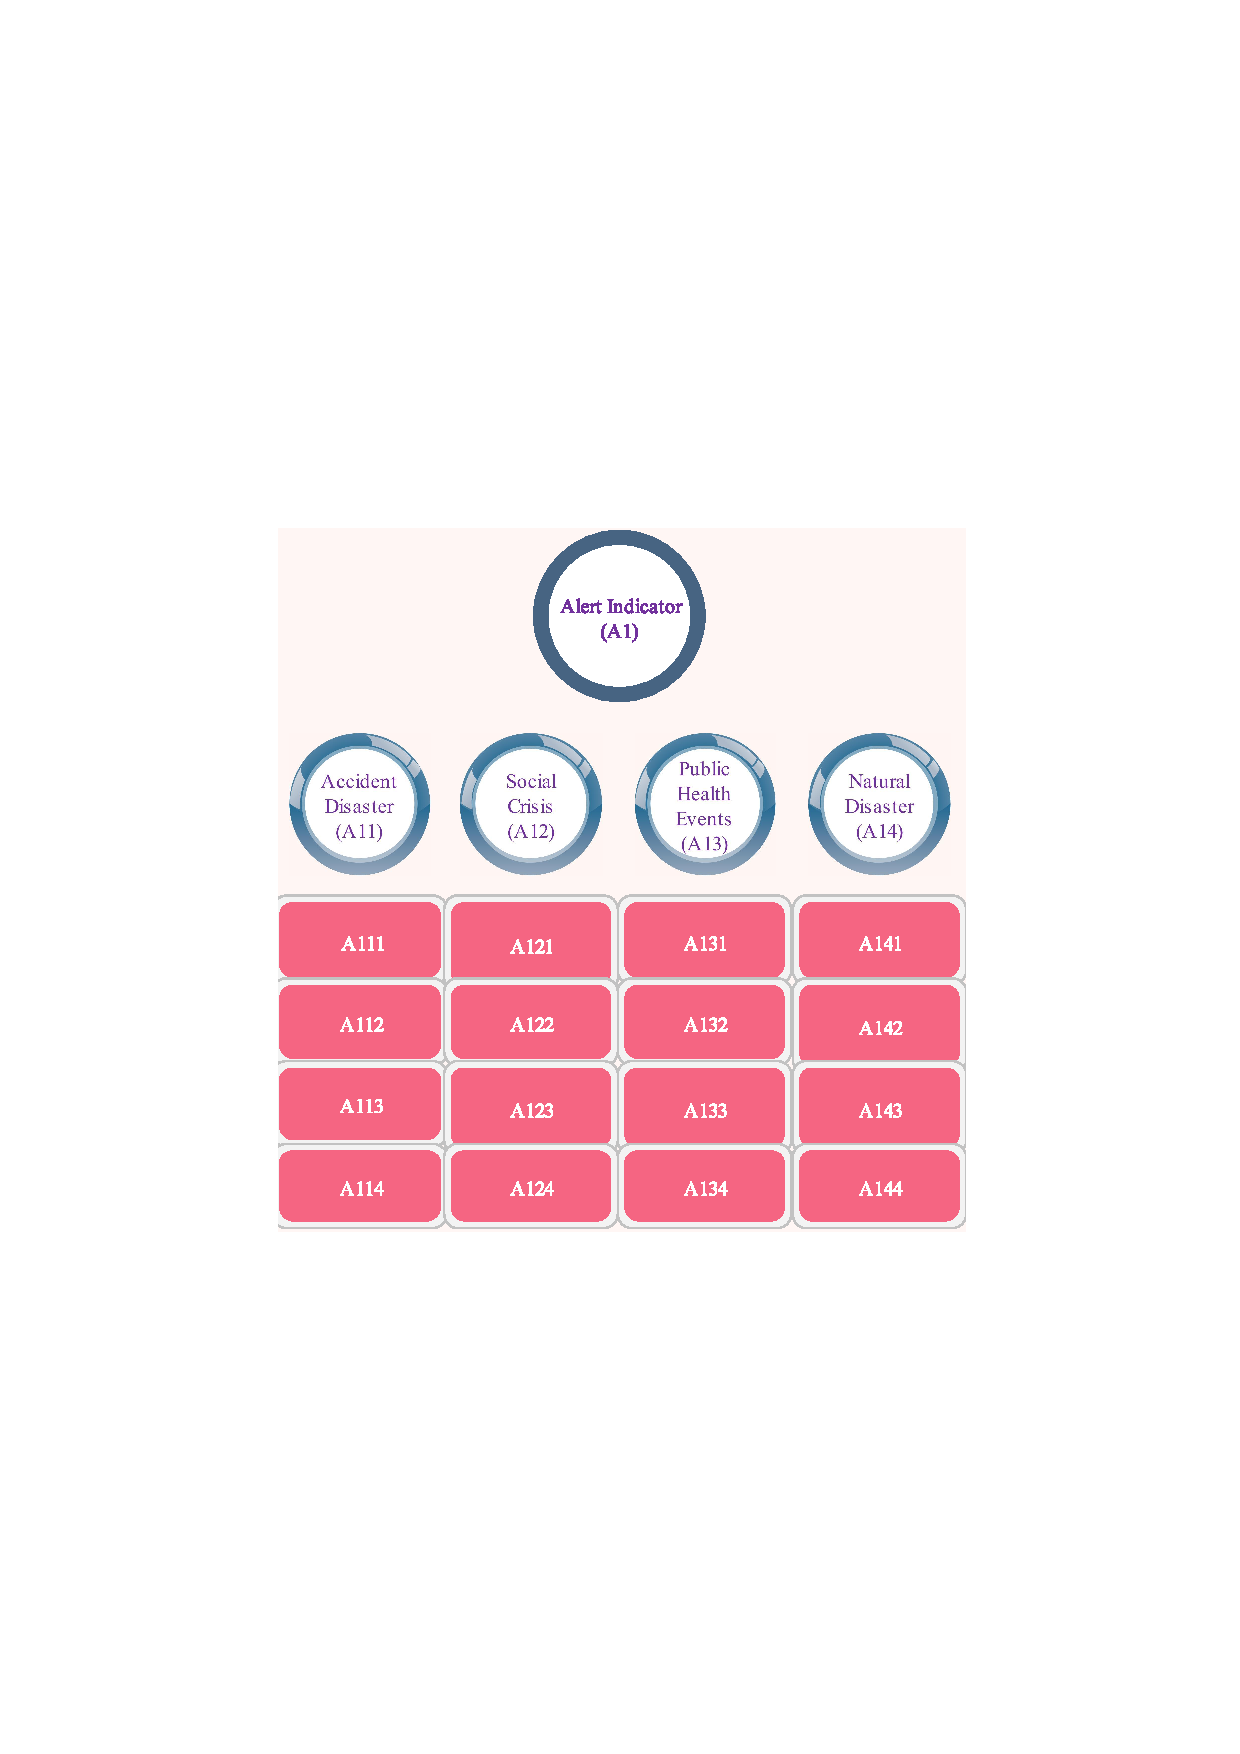
\includegraphics[width=\textwidth]{img/1.pdf}
% \end{subfigure}
% \begin{subfigure}[b]{.32\textwidth}
% 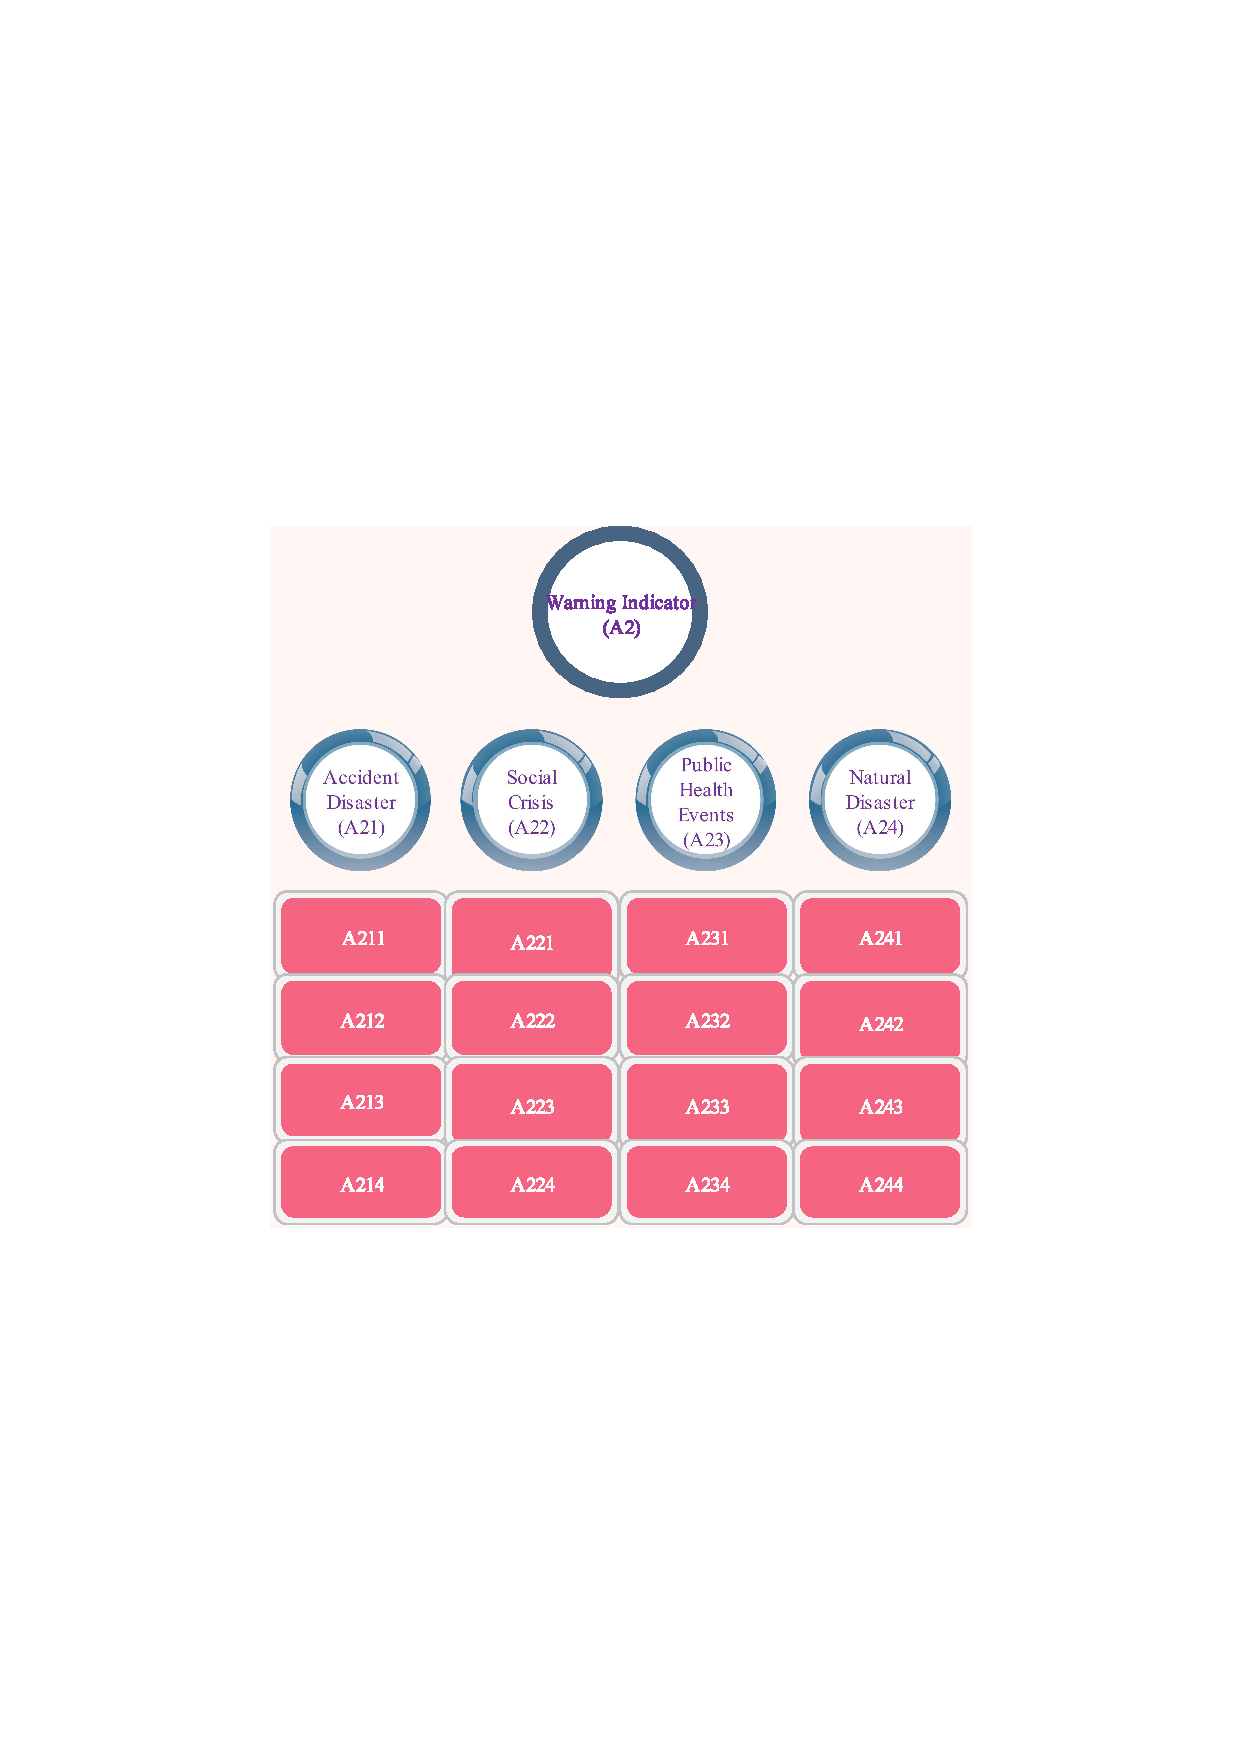
\includegraphics[width=\textwidth]{img/2.pdf}
% \end{subfigure}
% \begin{subfigure}[b]{.32\textwidth}
% 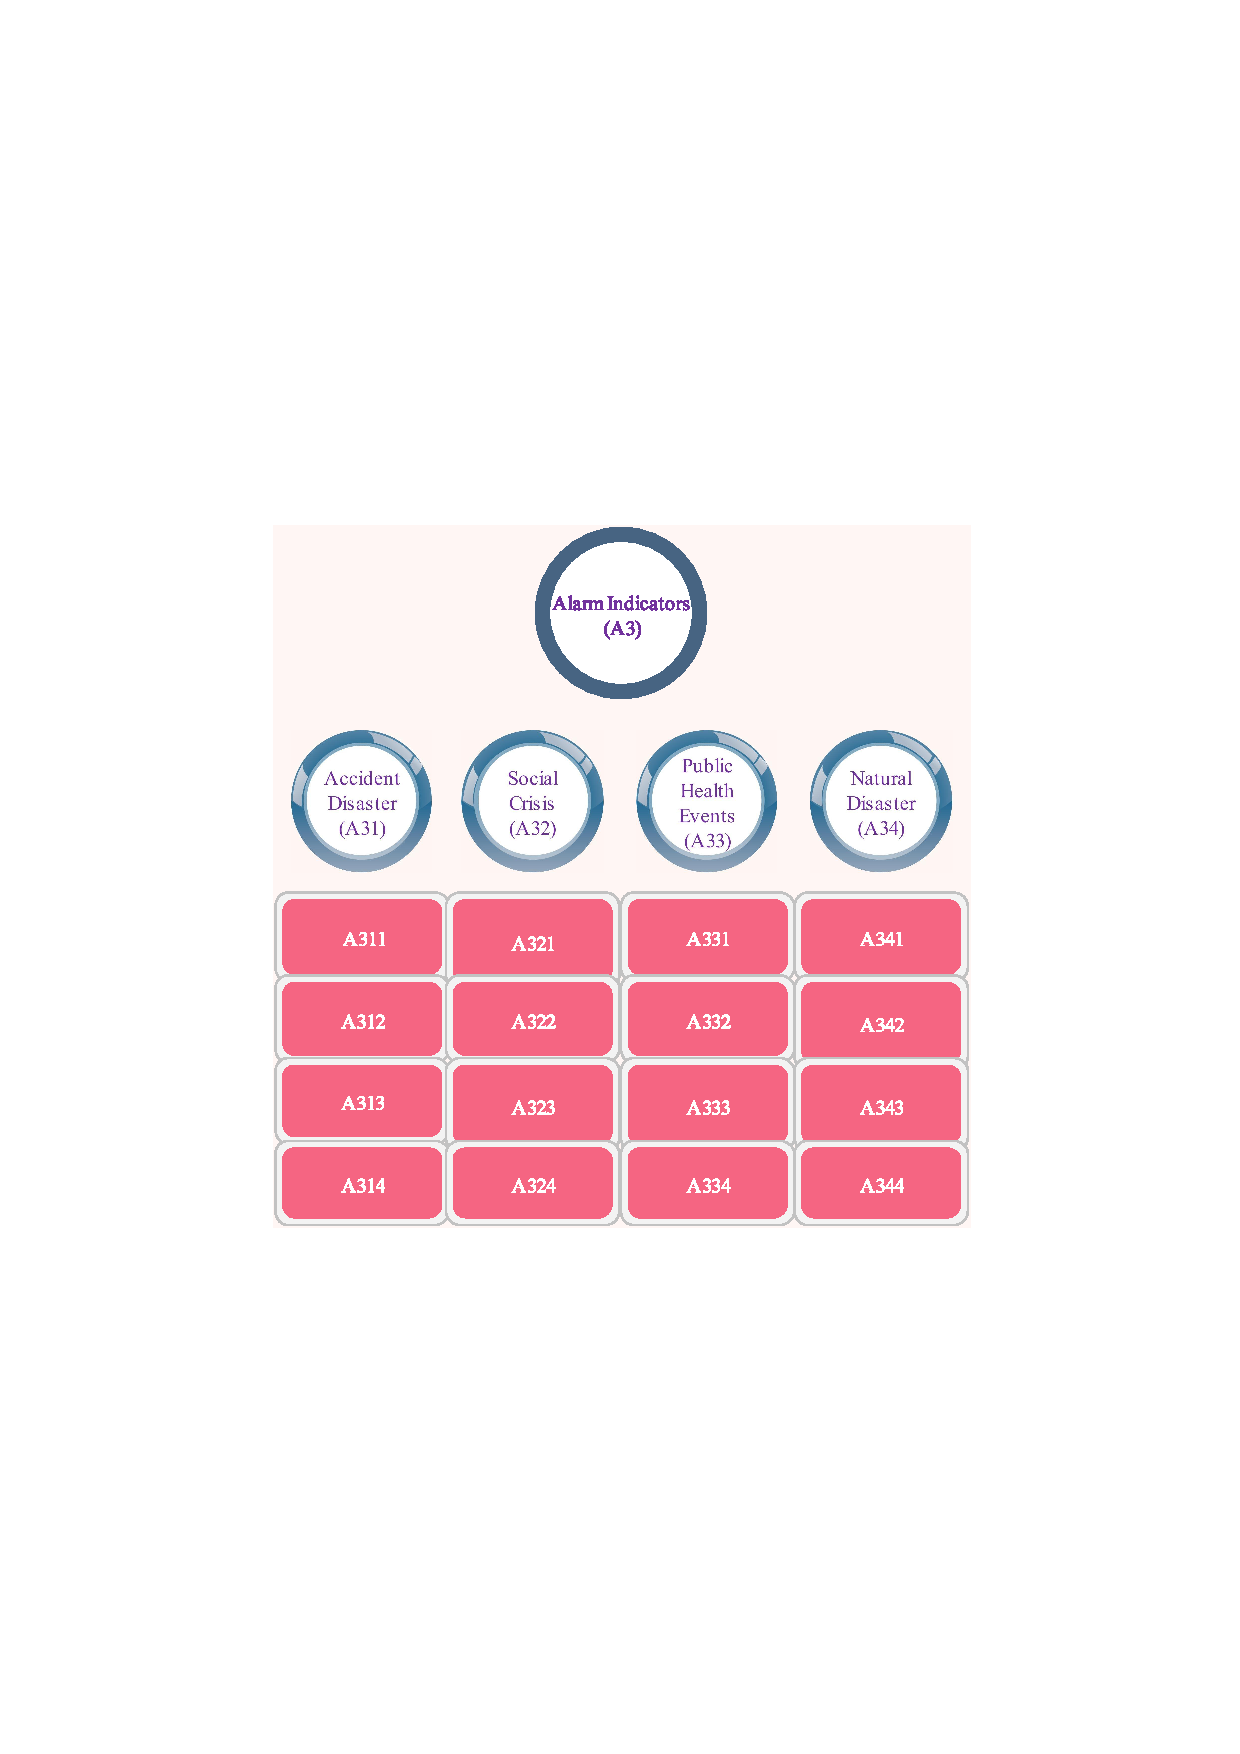
\includegraphics[width=\textwidth]{img/3.pdf}
% \end{subfigure}
% \caption{Your figure title}
% \end{figure}





\newpage
\section{Analysis and Promotion of Our Model}
\subsection{Sensitivity Analysis of Our Model}
\subsection{Strengths and Weaknesses}
Our research is basically based on the predecessors, and there are some improvements and shortcomings as follows:
\subsubsection{Strengths}
\subsubsection{Weaknesses}
\subsection{Future Work}























































% The instance of long and wide tables are shown in Table \ref{tb:longtable}.

% % 长表格示例,更多用法请参考 longtable 宏包文档
% % 以下环境及对应参数可实现表格内的自动换行与表格的自动断页
% % 您也可以选择自行载入 tabularx 宏包,并通过 X 参数指定对应列自动换行
% \begin{longtable}{ p{4em} p{14em} p{14em} }
% \caption{Basic Information about Three Main Continents (scratched from Wikipedia)}
% \label{tb:longtable}\\
% \toprule
% Continent & Description & Information \\
% \midrule
% Africa & Africa Continent is surrounded by the Mediterranean Sea to the
% north, the Isthmus of Suez and the Red Sea to the northeast, the Indian
% Ocean to the southeast and the Atlantic Ocean to the west. &
% At about 30.3 million km$^2$ including adjacent islands, it covers 6\%
% of Earth's total surface area and 20\% of its land area. With 1.3
% billion people as of 2018, it accounts for about 16\% of the world's
% human population. \\
% \midrule
% Asia & Asia is Earth's largest and most populous continent which
% located primarily in the Eastern and Northern Hemispheres.
% It shares the continental landmass of Eurasia with the continent
% of Europe and the continental landmass of Afro-Eurasia with both
% Europe and Africa. &
% Asia covers an area of 44,579,000 square kilometres, about 30\%
% of Earth's total land area and 8.7\% of the Earth's total surface
% area. Its 4.5 billion people (as of June 2019) constitute roughly
% 60\% of the world's population. \\
% \midrule
% Europe & Europe is a continent located entirely in the Northern
% Hemisphere and mostly in the Eastern Hemisphere. It comprises the
% westernmost part of Eurasia and is bordered by the Arctic Ocean to
% the north, the Atlantic Ocean to the west, the Mediterranean Sea to
% the south, and Asia to the east. &
% Europe covers about 10,180,000 km$^2$, or 2\% of the Earth's surface
% (6.8\% of land area), making it the second smallest
% continent. Europe had a total population of about 741 million (about
% 11\% of the world population) as of 2018. \\
% \bottomrule
% \end{longtable}
















% 以下为信件/备忘录部分,不需要可自行去掉
% 如有需要可将整个 letter 环境移动到文章开头或中间
% 请在第二个花括号内填写标题,如「信件」(Letter)或「备忘录」(Memorandum)
\begin{letter}{\huge{$\mathscr{MEMO}$}}
\begin{flushleft}  % 左对齐环境,无首行缩进
\textbf{To:} MCM/ICM organizing committee\\
\textbf{From:} Team 000000\\
\textbf{Date:}\today\\
\textbf{Subject:} 
\end{flushleft}
\lettrine{T}{he}
{\itshape \begin{enumerate}[0]
    \item[$\bullet$] Keep a firm grip on the local media to prevent public opinion from getting out of control. There is no substitute for the role of the media in regime change, and its entry into and occupation of a country's position of public opinion can help to bring down that country's regime. For the ruling party, therefore, to give ground. That means the beginning of the loss of power, public opinion out of control, not much time.
\end{enumerate}}
\end{letter}
\begin{algorithm}
\caption{Simulation-optimization heuristic}\label{algorithm}
\KwData{current period $t$, initial inventory $I_{t-1}$, initial capital $B_{t-1}$, demand samples}
\KwResult{Optimal order quantity $Q^{\ast}_{t}$}
$r\leftarrow t$\;
$\Delta B^{\ast}\leftarrow -\infty$\;
\While{$\Delta B\leq \Delta B^{\ast}$ and $r\leq T$}{$Q\leftarrow\arg\max_{Q\geq 0}\Delta B^{Q}_{t,r}(I_{t-1},B_{t-1})$\;
$\Delta B\leftarrow \Delta B^{Q}_{t,r}(I_{t-1},B_{t-1})/(r-t+1)$\;
\If{$\Delta B\geq \Delta B^{\ast}$}{$Q^{\ast}\leftarrow Q$\;
$\Delta B^{\ast}\leftarrow \Delta B$\;}
$r\leftarrow r+1$\;}
\end{algorithm}
%伪代码








% \begin{figure}[h!] 	
% \vspace{-0.8cm}   %调整图片与上文的垂直距离  
% \setlength{\abovecaptionskip}{0.cm} %调整标题上方的距离   
% \setlength{\abovecaptionskip}{0.cm} %调整标题下方的距离 	   
% \setlength{\belowdisplayskip}{0.pt} 	
% 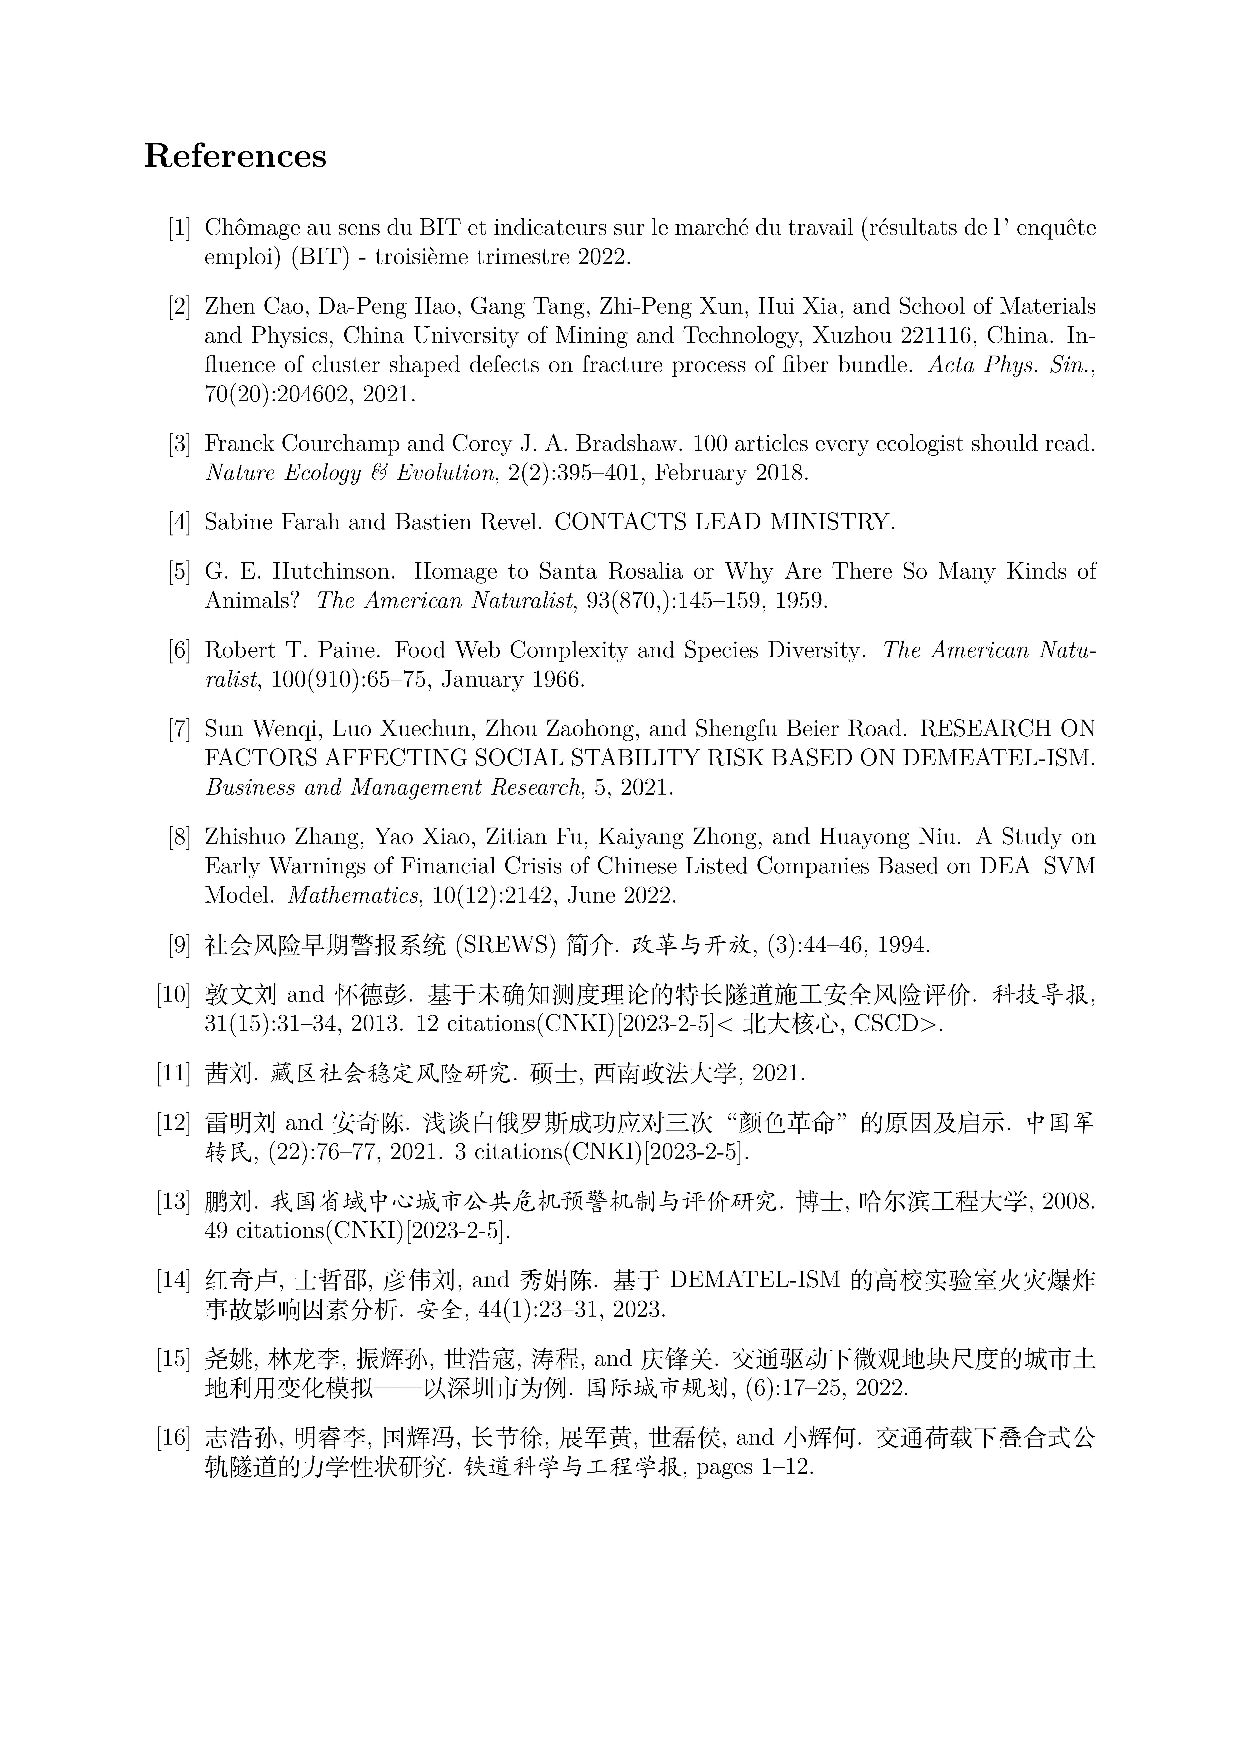
\includegraphics[width=15cm]{img/c1.pdf}  
% \end{figure}
% \newpage
% \begin{figure}[h!] 	
% \vspace{-0.8cm}   %调整图片与上文的垂直距离   
% \setlength{\belowdisplayskip}{10.pt} 	
% 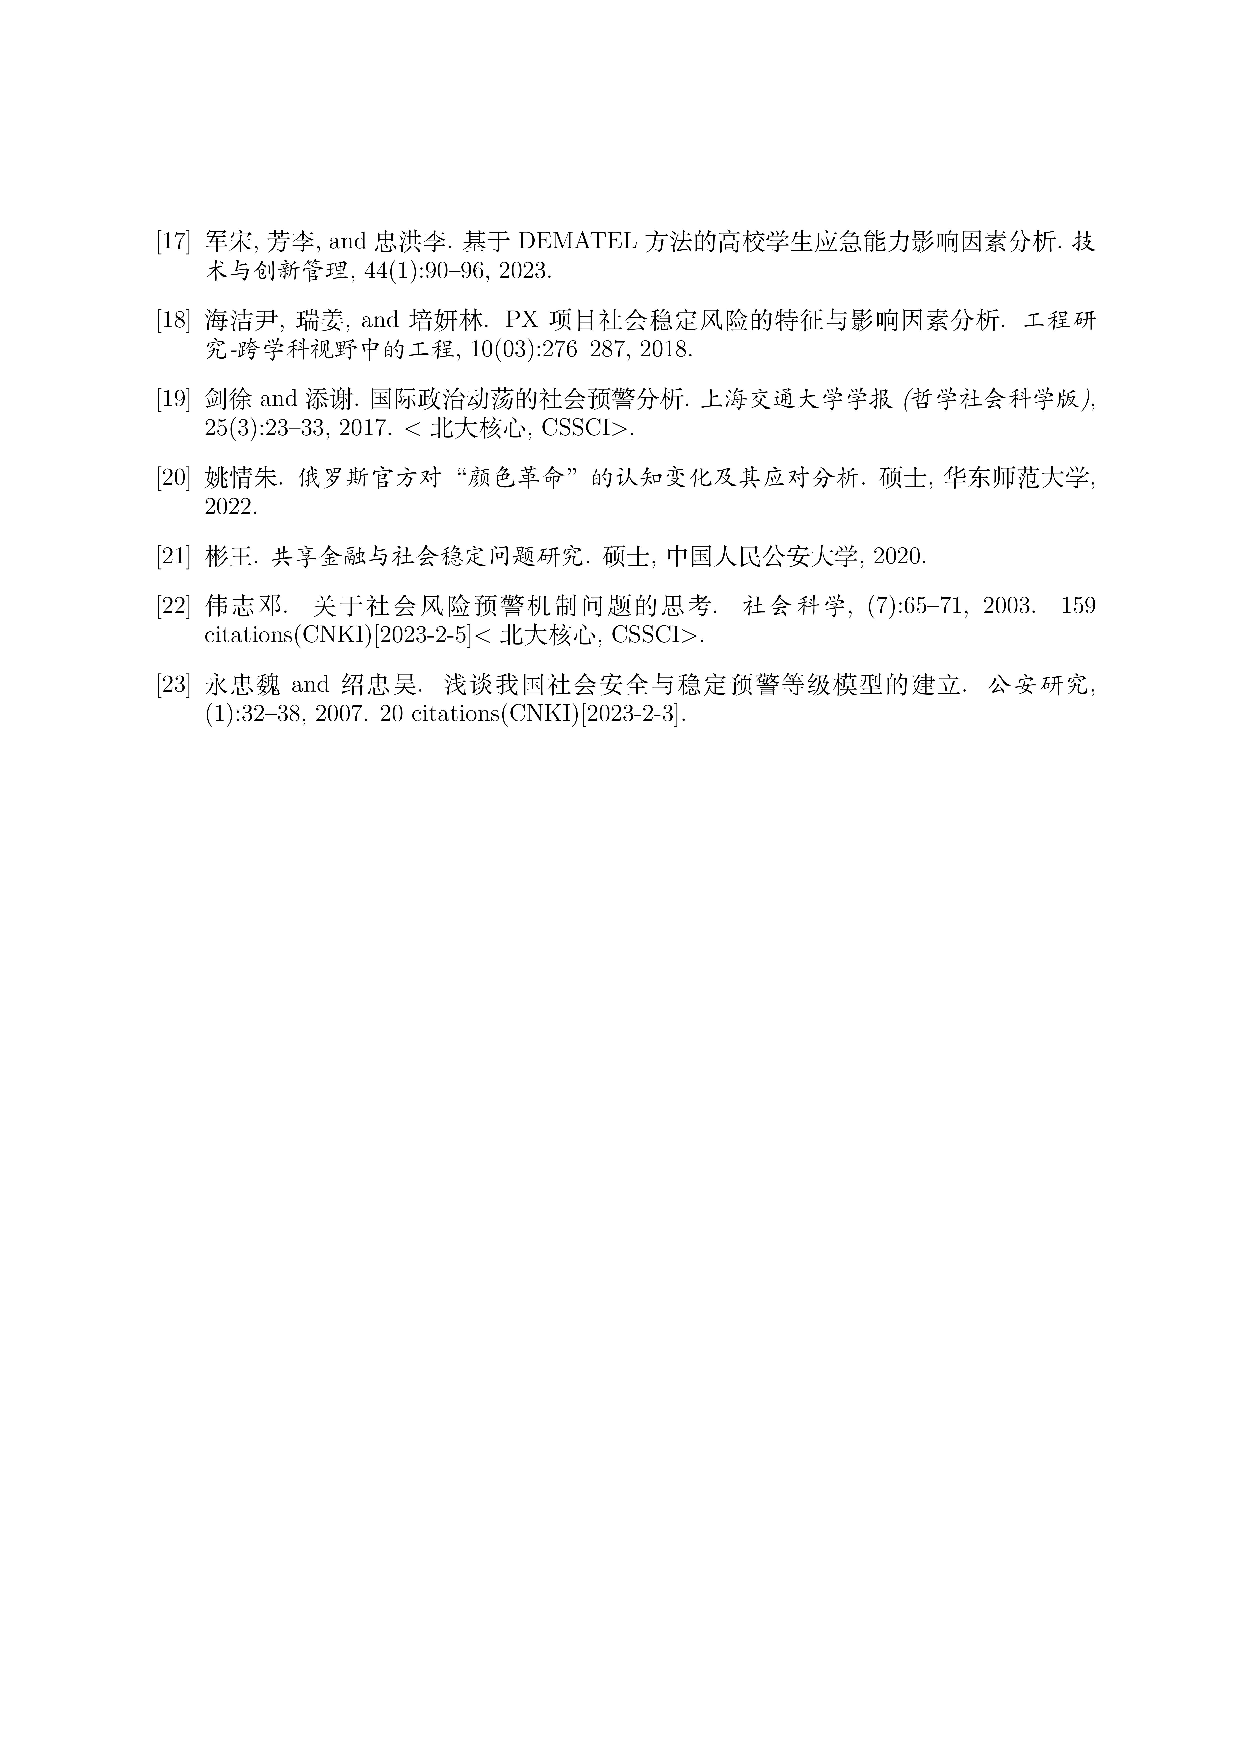
\includegraphics[width=15cm]{img/c2.pdf}  
% \end{figure}











\newpage
% 参考文献,此处以 MLA 引用格式为例
\begin{thebibliography}{100}

\bibitem{noauthor_chomage_nodate}
Chômage au sens du {BIT} et indicateurs sur le marché du travail (résultats
  de l’enquête emploi) ({BIT}) - troisième trimestre 2022.
\end{thebibliography}



% 以下为附录内容
% 如您的论文中不需要附录,请自行删除
\begin{subappendices}  % 附录环境
\section{Appendix}


\end{subappendices}  % 附录内容结束



















































\end{document}  % 结束
